\chapter{Pruebas y resultados}
\label{chap:pruebas_y_resultados}

En este capítulo se presentan las pruebas realizadas para comprobar el funcionamiento del simulador y analizar los resultados obtenidos en distintos casos de estudio.


\section{Escenario de pruebas}

Las pruebas se realizan sobre el escenario tridimensional del Centro Universitario de Mérida descrito en capítulos anteriores. La antena transmisora se mantiene en la parte superior del edificio administrativo, siguiendo la ubicación real tomada como referencia.

La configuración mostrada en la Tabla \ref{tab:parametros} se utiliza como caso base para el resto de pruebas. A partir de ella, se modifican algunos parámetros concretos, como el método de reconstrucción del patrón de radiación, el valor de k en el método de Vasiliadis y la potencia de transmisión.

\begin{table}[H]
    \centering
    \begin{tabularx}{\textwidth}{@{}llX@{}}
        \toprule
        \textbf{Parámetro} & \textbf{Valor}\\
        \midrule
        \texttt{Método de reconstrucción} & Vasiliadis, k = 2 \\
        \texttt{Potencia del transmisor} & 30 dBm \\
        \texttt{Frecuencia} & 1,785 GHz \\
        \texttt{Ancho de banda} & 10 MHz \\
        \texttt{Modelo de pérdidas} & FSPL \\
        \texttt{Shadowing} & Desactivado \\
        \texttt{Tamaño de la rejilla} & 300 x 40 x 400 m \\
        \texttt{Tamaño del vóxel} & 2 m \\
        \texttt{Ganancia receptores vehiculares} & 3 dBi \\
        \texttt{Ganancia receptor celular} & 0 dBi \\
        \bottomrule
    \end{tabularx}
    \caption{Parámetros de prueba}
    \label{tab:parametros}
\end{table}

La antena utilizada en el simulador es el modelo HWXX-6516DS1-VTM de Andrew. Según su ficha técnica, la antena trabaja en varias bandas dentro del rango de 1710 a 2690 MHz y admite una potencia máxima de 350 W por puerto~\cite{andrew_hwxx_datasheet}. Esta potencia máxima equivale aproximadamente a:

\[
P_{\mathrm{tx}}(\mathrm{dBm}) = 10 \log_{10}(350000) \approx 55,44\ \mathrm{dBm}
\]

En las pruebas no se utiliza la potencia máxima admitida por la antena, ya que este valor representa el límite físico que puede soportar el puerto de entrada y no una potencia habitual. En su lugar, se utiliza una potencia de transmisión de 30 dBm, equivalente a 1 W, como caso base para el escenario del campus. Este valor es inferior al límite indicado para una estación base de rango medio en ETSI TS 138 104, donde se define para las estaciones de rango medio una potencia menor o igual a 38 dBm \cite{etsi138104}. Además, al estar muy por debajo de los 350 W por puerto indicados en la ficha técnica, el valor seleccionado queda dentro del margen soportado por la antena.

La frecuencia seleccionada es 1,785 GHz. En la página del fabricante se encuentran disponibles distintos ficheros CSV con patrones de radiación medidos para varias frecuencias de operación de la antena \cite{andrew_hwxx_product}. En el simulador se utiliza el fichero correspondiente a 1,785 GHz. De esta forma, la frecuencia utilizada en los cálculos coincide con la frecuencia del patrón de radiación reconstruido.

El ancho de banda para todos los receptores es de 10 MHz. Este valor aparece tanto en las configuraciones de canal de 5G NR en FR1 \cite{etsi138104} como en comunicaciones vehiculares V2X \cite{etsi302663}. Como ambos casos pueden utilizar este ancho de banda, se ha utilizado el mismo valor para los receptores celulares y vehiculares, evitando diferentes anchos de banda en cada tipo de receptor.

Como modelo de pérdidas se utiliza FSPL. Se ha elegido este modelo como base para hacer todas las pruebas porque representa la propagación en espacio libre y permite comprobar los resultados de forma sencilla mediante fórmulas teóricas.

El \textit{shadowing} se desactiva en la configuración para garantizar que las simulaciones sean reproducibles. Al eliminar la componente aleatoria, dos ejecuciones con los mismos parámetros producen los mismos resultados, lo que facilita la validación del simulador y la comparación entre configuraciones.

La rejilla de simulación tiene un tamaño de $300 \times 40 \times 400$ m. Estas dimensiones son las mínimas para cubrir el campus al completo y poder analizar el mapa de calor en todo el escenario. Debido al gran tamaño de la rejilla, se utiliza un tamaño de vóxel de 2 m, ya que en caso de ser más pequeño el número de muestras sería excesivo para un ordenador de uso personal. En las pruebas donde se comparan mapas de calor a la altura del suelo se aumenta el alto de la rejilla de 40 a 50 para tener un margen más amplio.

En los receptores vehiculares se emplea una ganancia de 3 dBi, tomando como referencia los supuestos de simulación utilizados en estudios V2X de 3GPP~\cite{tr36885}. Para el receptor celular se utiliza una ganancia de 0 dBi para modelarlo como un terminal de usuario genérico. Este valor se toma como referencia a partir de ETSI TR 136 942~\cite{etsi136942}.

A partir de este caso base, se analizan variaciones según el patrón de radiación y la potencia de transmisión, observando su impacto sobre la potencia recibida, la SNR y la cobertura obtenida en el campus.

\section{Validación del patrón de radiación reconstruido}

Antes de utilizar el patrón de radiación en los cálculos de propagación, se realiza una prueba para comprobar que la reconstrucción implementada en Unity se ha realizado correctamente.

Para realizar esta comprobación, se crearon bolas de \textit{debug} dentro del simulador. Estas bolas se sitúan en el centro de cada vóxel de la rejilla y se utilizan únicamente durante las pruebas internas de desarrollo, por lo que el usuario final desconocerá su existencia. Su objetivo es permitir la inspección de los valores calculados en puntos concretos del escenario y comprobar que la reconstrucción del patrón de radiación funciona correctamente.

En la Figura \ref{fig:bolas_debug} se muestra un ejemplo de estas bolas de \textit{debug} colocadas sobre la rejilla de simulación. Cada bola representa un punto de la rejilla que puede seleccionarse para consultar los valores calculados en esa posición.

\begin{figure}[H]
    \centering
    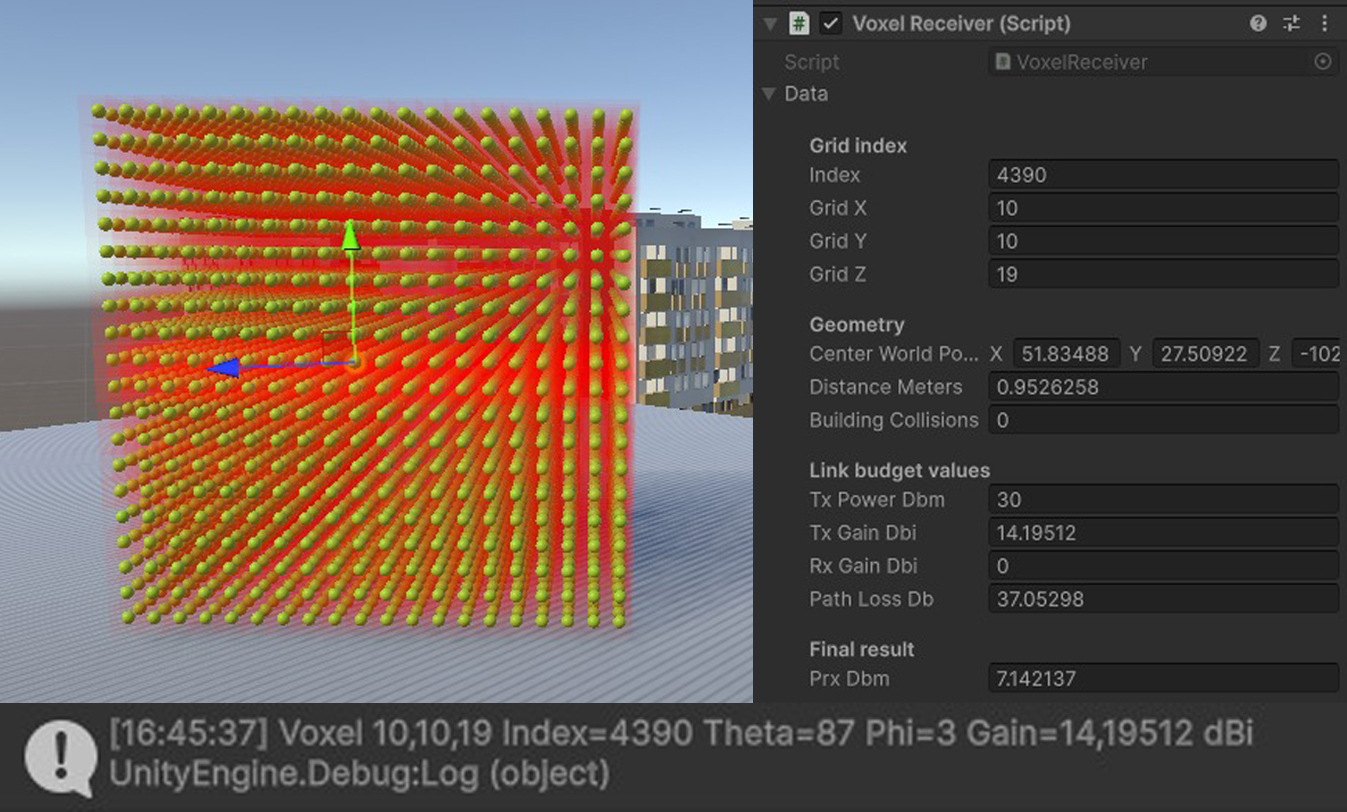
\includegraphics[width=0.85\textwidth, keepaspectratio]{imagenes/resultados/patron de radiacion/Bolas debug.jpg}
    \caption{Bolas de \textit{debug} utilizadas para inspeccionar valores de la rejilla}
    \label{fig:bolas_debug}
\end{figure}

Al hacer clic en una de estas bolas, el simulador muestra la información asociada a ese vóxel. Además, durante la generación de la rejilla, Unity muestra por consola un mensaje con el índice de cada bola y los ángulos theta y phi correspondientes a la dirección entre la antena y ese punto. Esta información permite realizar dos comprobaciones: por un lado, validar el cálculo de potencia recibida mediante el presupuesto de potencias y, por otro, comprobar que la ganancia del patrón de radiación se obtiene correctamente para esa dirección.

En primer lugar, se verifica el cálculo de potencia recibida en un punto concreto. Para ello, se utiliza la bola de \textit{debug} de la Figura \ref{fig:bolas_debug}, cuyo panel muestra una potencia recibida de $7,14$ dBm. Al tratarse de una prueba con el modelo FSPL y sin \textit{shadowing}, este valor puede comprobarse fácilmente mediante la expresión de pérdidas en el espacio libre \cite{itur_p341}:

\[
L_{\mathrm{FSPL}}(\mathrm{dB}) = 20 \log_{10}\left(\frac{4 \pi d f}{c}\right)
\]


donde $d$ es la distancia entre el transmisor y el receptor en metros, $f$ es la frecuencia en Hz y $c$ es la velocidad de la luz en m/s. A partir de esta pérdida, la potencia recibida se obtiene mediante el presupuesto de potencias:

\[
P_{\mathrm{rx}} = P_{\mathrm{tx}} + G_{\mathrm{tx}} + G_{\mathrm{rx}} - L_{\mathrm{FSPL}} - L_{\mathrm{edificios}}
\]

Para el punto seleccionado, el simulador muestra una distancia de $0,95$ m, una ganancia de transmisión de $14,20$ dBi, una ganancia de recepción de $0$ dBi y cero colisiones con edificios. Por tanto, las pérdidas adicionales por edificios son $0$ dB. Sustituyendo estos valores:

\[
L_{\mathrm{FSPL}} = 20 \log_{10}\left(\frac{4 \pi \cdot 0,95 \cdot 1,785 \cdot 10^9}{3 \cdot 10^8}\right) = 37,05\ \mathrm{dB}
\]

\[
P_{\mathrm{rx}} = 30 + 14,20 + 0 - 37,05 - 0 = 7,15\ \mathrm{dBm}
\]

Este valor coincide con el mostrado en la bola de \textit{debug}, donde se obtiene una potencia recibida de $7,14$ dBm. Esta comprobación permite verificar que el cálculo de pérdidas y el presupuesto de potencias se están aplicando correctamente.

Una vez comprobado el cálculo de potencia recibida, se validan las ganancias del patrón de radiación. Para ello, se utilizan los ángulos theta y phi asociados a cada bola de \textit{debug} y se comparan con una reconstrucción equivalente realizada en MATLAB mediante la función \texttt{patternFromSlices} \cite{mathworks_patternfromslices}. Así, para cada bola seleccionada, se compara la ganancia calculada por Unity con la ganancia obtenida en MATLAB para el mismo par de ángulos.

La comparación se realizó utilizando el método de Vasiliadis con dos valores distintos del parámetro $k$. Por un lado, se realizaron pruebas con $k = 1$ para observar el comportamiento de la reconstrucción con una ponderación más suave. Por otro lado, con $k = 2$, que es el valor utilizado como configuración base en el resto de pruebas del simulador.

En la Tabla \ref{tab:comprobacion_patron} se muestran los valores obtenidos para distintos pares de ángulos. Para cada dirección se incluye la ganancia calculada en MATLAB y los valores obtenidos en Unity con Vasiliadis para $k = 1$ y $k = 2$.

\begin{table}[H]
    \centering
    \begin{tabularx}{\textwidth}{@{}ccXXX@{}}
        \toprule
        \textbf{$\theta$} & \textbf{$\phi$} & \textbf{MATLAB (dBi)} & \textbf{Unity $k=1$ (dBi)} & \textbf{Unity $k=2$ (dBi)}\\
        \midrule
        90 & 25 & 14,25 & 14,25 & 14,25 \\
        90 & 68 & 6,80 & 6,80 & 6,80 \\
        90 & 180 & -18,82 & -18,82 & -18,82 \\
        135 & 0 & 3,71 & 3,70 & -3,71 \\
        87 & 3 & 14,20 & 14,34 & 14,20 \\ % 4390
        48 & 245 & -15,77 & -7,38 & -15,77 \\ % 7700
        93 & 165 & -19,89 & -19,88 & -19,89 \\ % 3612
        138 & 315 & 0,63 & -1,30 & 0,63 \\ % 704
        72 & 65 & -10,37 & -9,97 & -10,37 \\ % 5499
        168 & 198 & -28,03 & -14,97 & -28,03 \\ % 969
        \bottomrule
    \end{tabularx}
    \caption{Comparación de ganancias del patrón reconstruido}
    \label{tab:comprobacion_patron}
\end{table}

Los resultados muestran que los valores obtenidos en Unity con el método de Vasiliadis y $k = 2$ coinciden con los obtenidos en MATLAB para los ángulos analizados. Esto confirma que la implementación utilizada en el simulador reproduce correctamente la reconstrucción tomada como referencia. En cambio, al utilizar $k = 1$ se obtiene un rango de ganancias más reducido entre los valores máximos y mínimos, por lo que el patrón reconstruido presenta variaciones más leves. Por este motivo, se utiliza $k = 2$ como valor base en el resto de pruebas.

Además, los primeros ángulos de la tabla son direcciones pertenecientes a los cortes horizontal y vertical del fichero CSV original, por lo que no dependen de la reconstrucción. Estos casos sirven como comprobación de que la lectura del fichero de antena y la conversión de ángulos utilizada en Unity son correctas. Los valores obtenidos coinciden con los del CSV original, lo que confirma que el simulador funciona correctamente.

En la Figura \ref{fig:patron_matlab} se muestra visualmente la comparación entre el patrón reconstruido en Unity mediante el método de Vasiliadis con $k = 2$ y el patrón obtenido en MATLAB. En ambos casos se aprecia una forma muy similar del lóbulo principal y de las zonas de menor ganancia, lo que confirma que la reconstrucción no solo coincide en los puntos numéricos comprobados, sino también en la forma general del patrón tridimensional.

\begin{figure}[H]
    \centering
    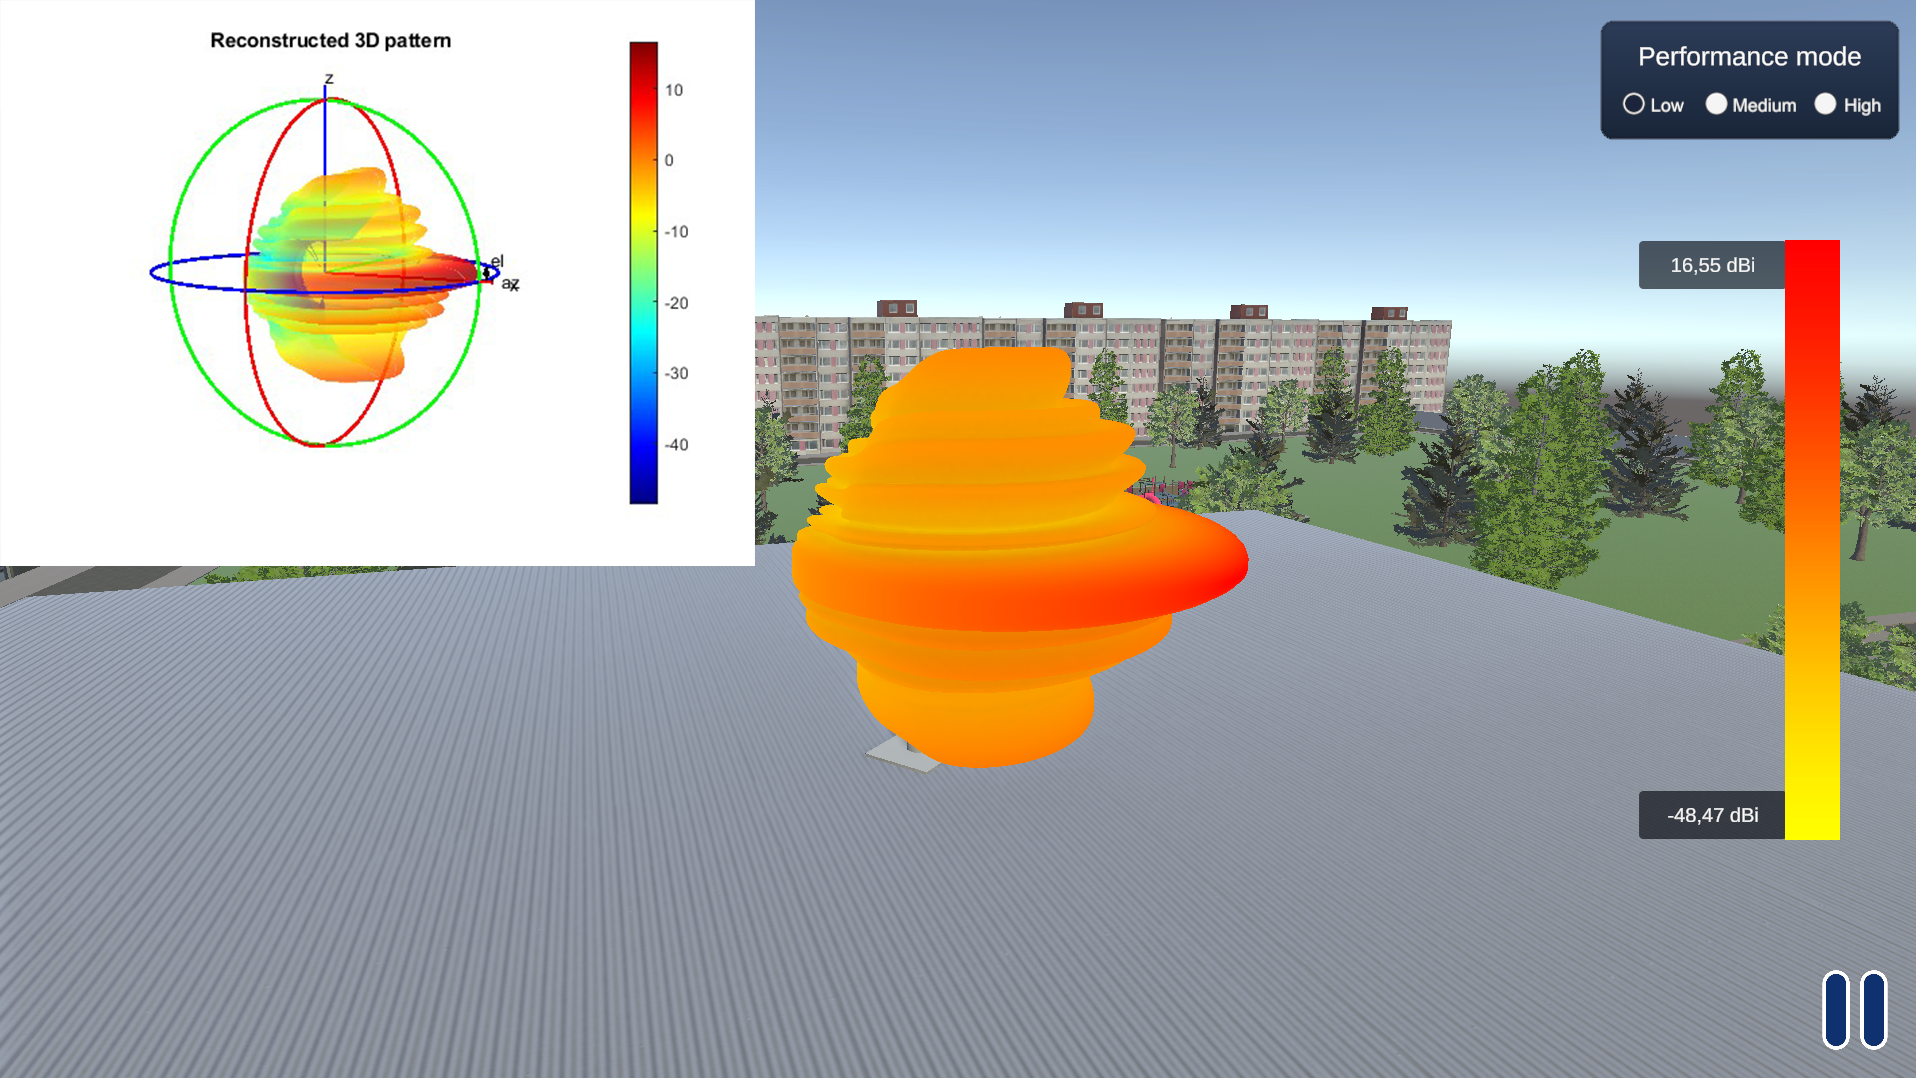
\includegraphics[width=1\textwidth, keepaspectratio]{imagenes/resultados/patron de radiacion/patron de radiacion.PNG}
    \caption{Comparación del patrón reconstruido con el de MATLAB}
    \label{fig:patron_matlab}
\end{figure}

Esta prueba también permite validar que la conversión entre posiciones del escenario y ángulos del patrón se realiza correctamente. Por tanto, el patrón reconstruido puede utilizarse posteriormente en los cálculos de propagación, ya que el simulador es capaz de obtener la ganancia de transmisión correspondiente a cada dirección del espacio.


\section{Resultados rejilla de propagación}

En esta sección se muestran los resultados obtenidos al calcular la rejilla tridimensional de vóxeles. En primer lugar, se representa una rejilla reducida de $50 \times 40 \times 50$ m, ya que este tamaño permite apreciar con claridad la distribución de la potencia recibida alrededor de la antena. Al ser el número total de vóxeles muy reducido, se puede apreciar fácilmente sin necesidad de utilizar el umbral o el mapa en dos dimensiones.

En la Figura \ref{fig:heatmap_3d_reducido} se puede ver cómo la potencia recibida no se distribuye de forma uniforme en todas las direcciones. Las zonas con mayor intensidad de rojo se corresponden con las zonas de mayor potencia recibida, mientras que las zonas más alejadas o en direcciones de bajas ganancias en el patrón de radiación tienen valores más oscuros y transparentes.

\begin{figure}[H]
    \centering
    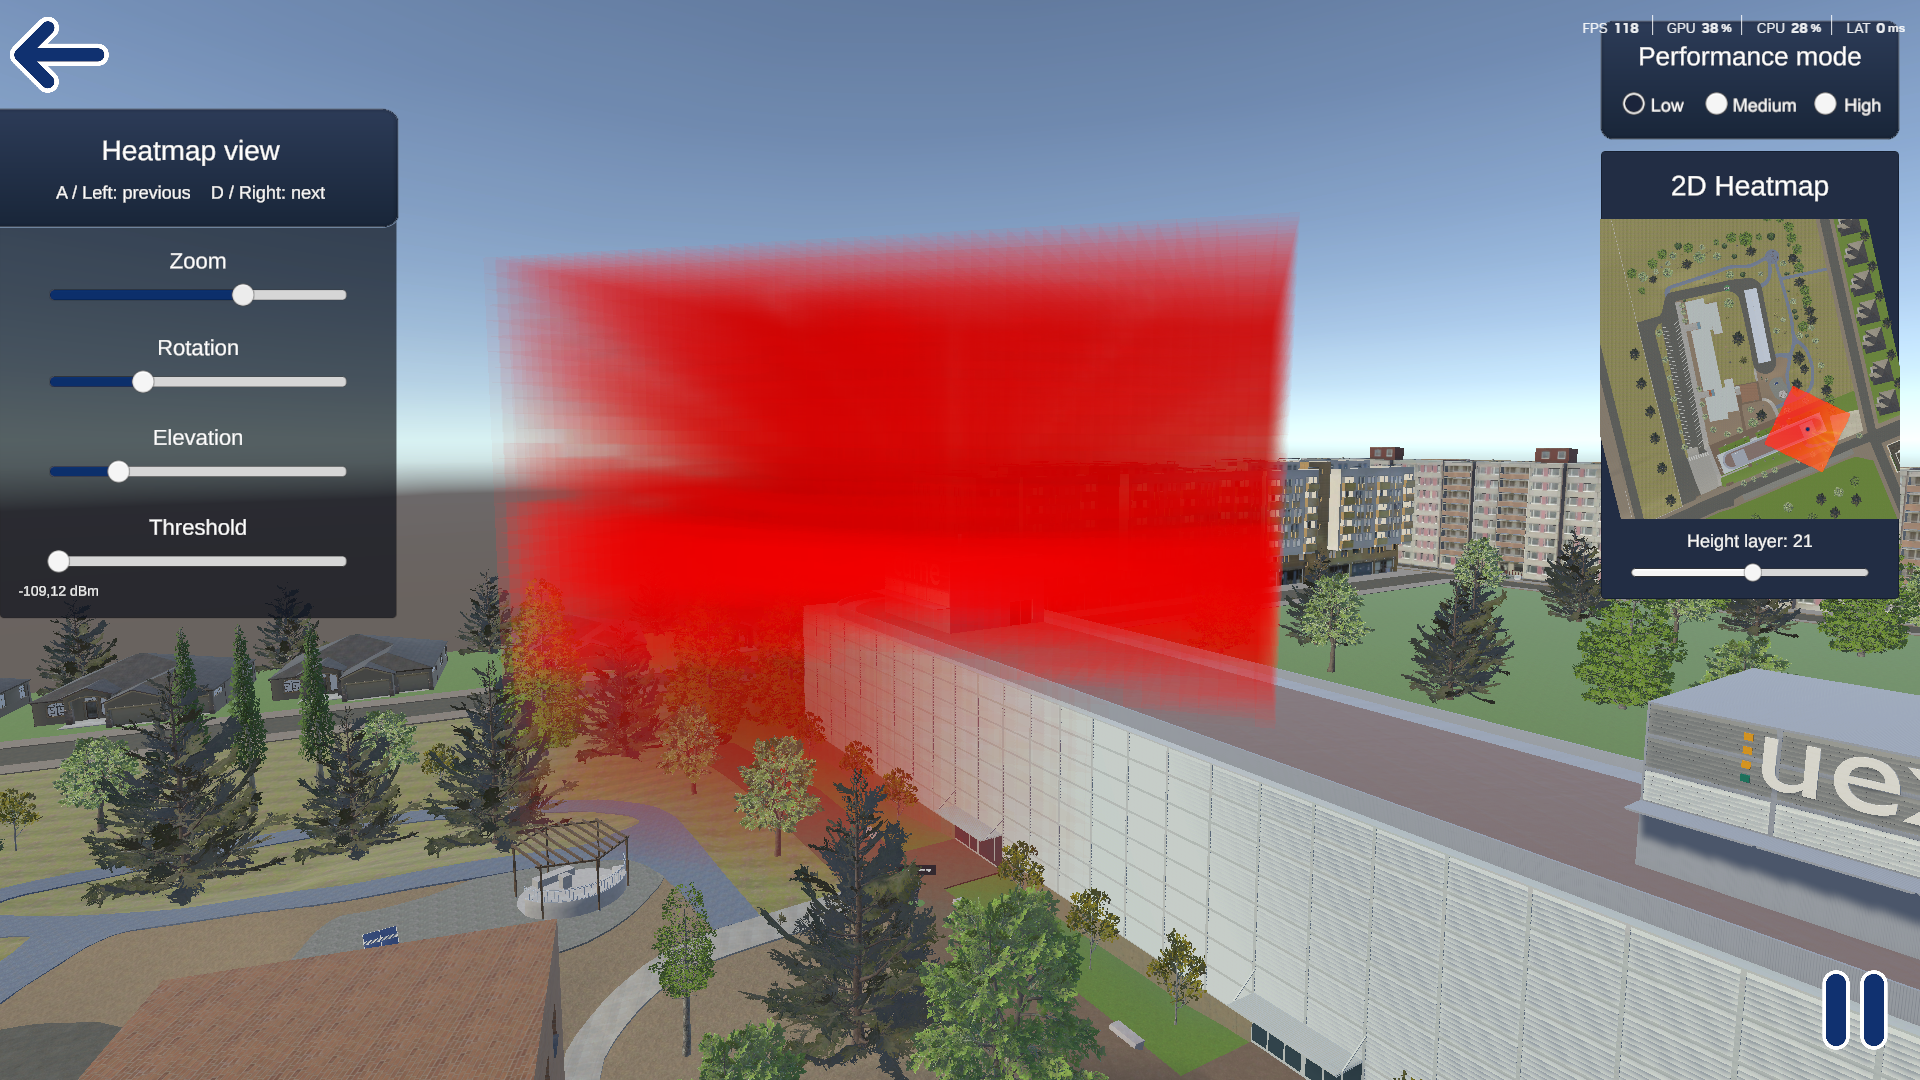
\includegraphics[width=1\textwidth, keepaspectratio]{imagenes/resultados/mapas de calor/Mapa de calor 50x40x50.PNG}
    \caption{Mapa de calor 3D para una rejilla reducida de $50 \times 40 \times 50$ m}
    \label{fig:heatmap_3d_reducido}
\end{figure}

Sin embargo, cuando se utiliza la rejilla del caso base para cubrir todo el campus, la visualización tridimensional contiene un número mucho mayor de vóxeles. En este caso, aunque el resultado sigue siendo útil para observar la cobertura general, la densidad de puntos dificulta la interpretación directa del mapa completo.

Como se observa en la Figura \ref{fig:heatmap_3d_campus}, al representar todo el campus, el número de vóxeles aumenta considerablemente y la visualización resulta imposible de analizar. Por este motivo, en la siguiente representación se hace uso del umbral de visualización, ocultando los vóxeles con menor potencia recibida y manteniendo visibles únicamente las zonas con valores más altos.

\begin{figure}[H]
    \centering
    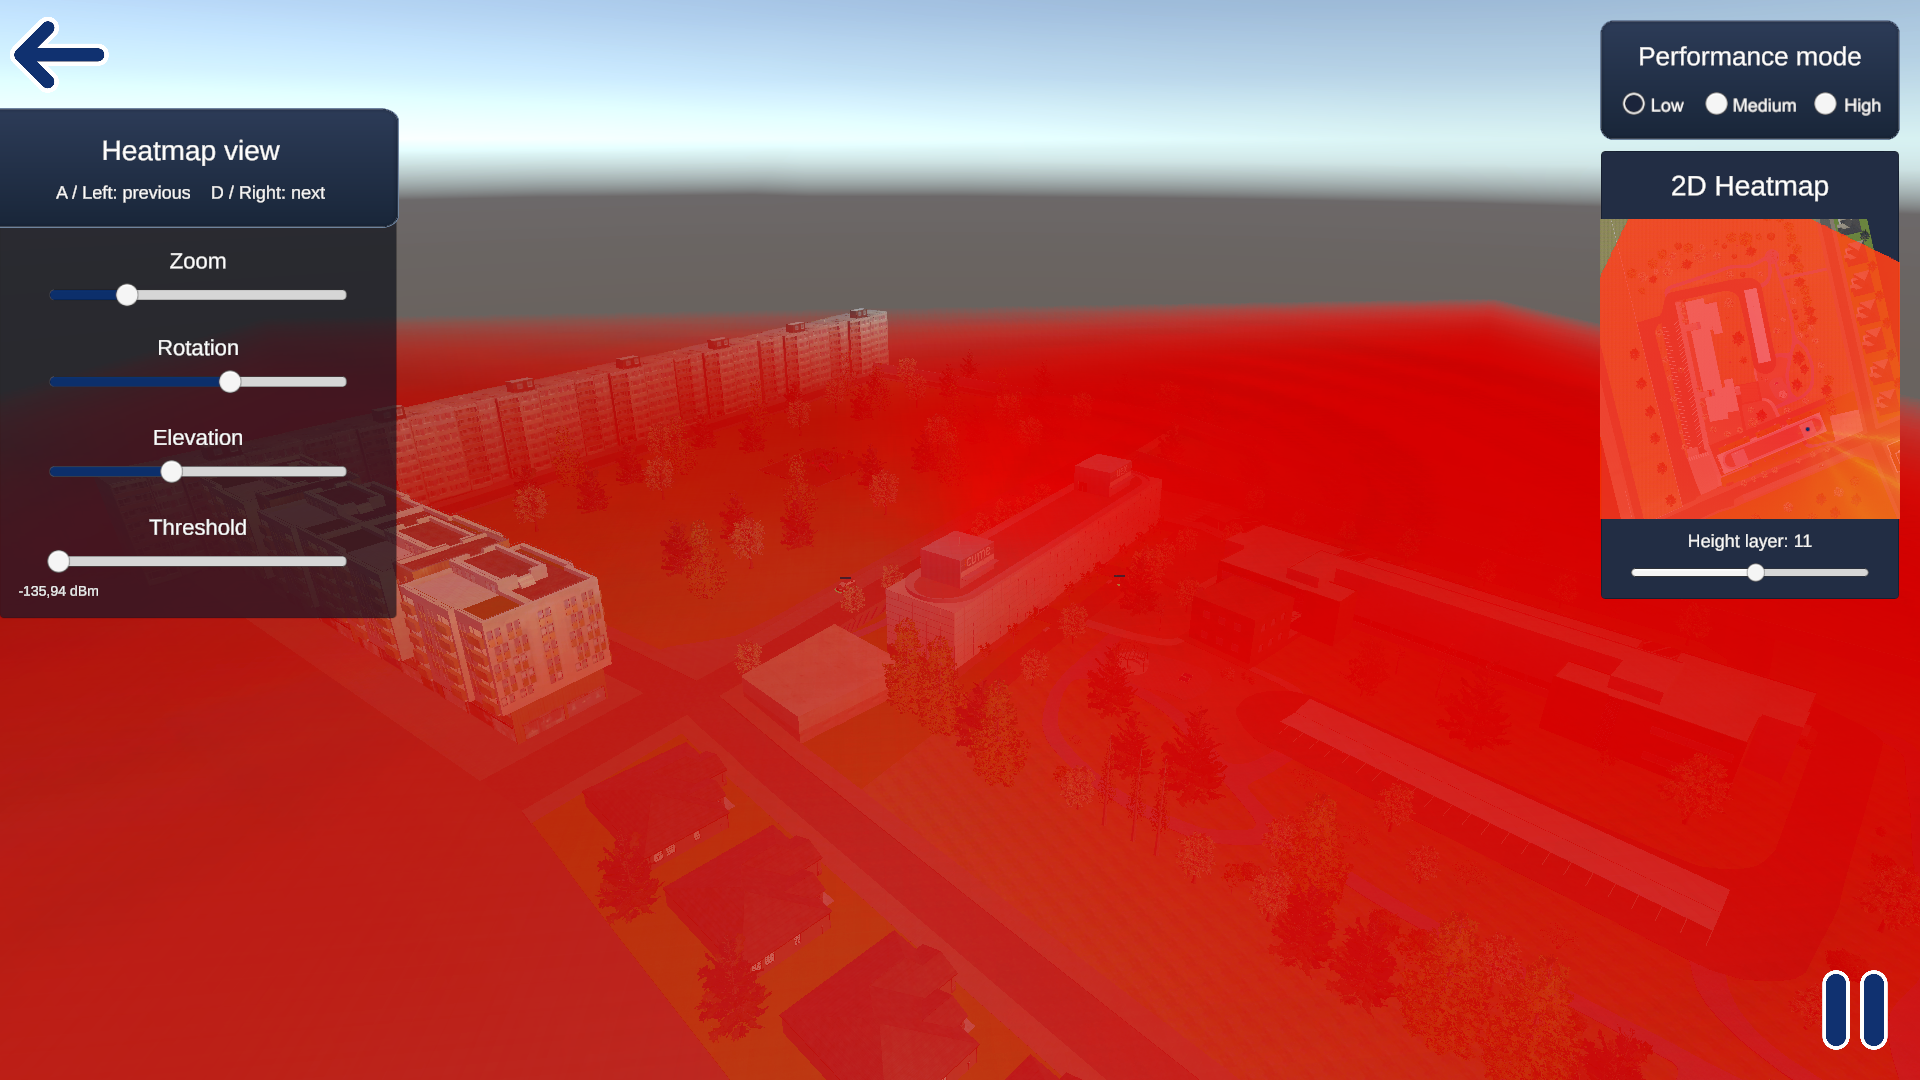
\includegraphics[width=1\textwidth, keepaspectratio]{imagenes/resultados/mapas de calor/Mapa de calor saturado.PNG}
    \caption{Mapa de calor 3D para la rejilla completa del campus}
    \label{fig:heatmap_3d_campus}
\end{figure}

En la Figura \ref{fig:heatmap_3d_umbral} se muestra cómo el uso del umbral facilita la visualización de las zonas con mayor potencia recibida. Esta representación permite distinguir con mayor claridad las regiones principales de cobertura, especialmente alrededor de la antena y en las direcciones donde el patrón de radiación presenta una mayor ganancia.

\begin{figure}[H]
    \centering
    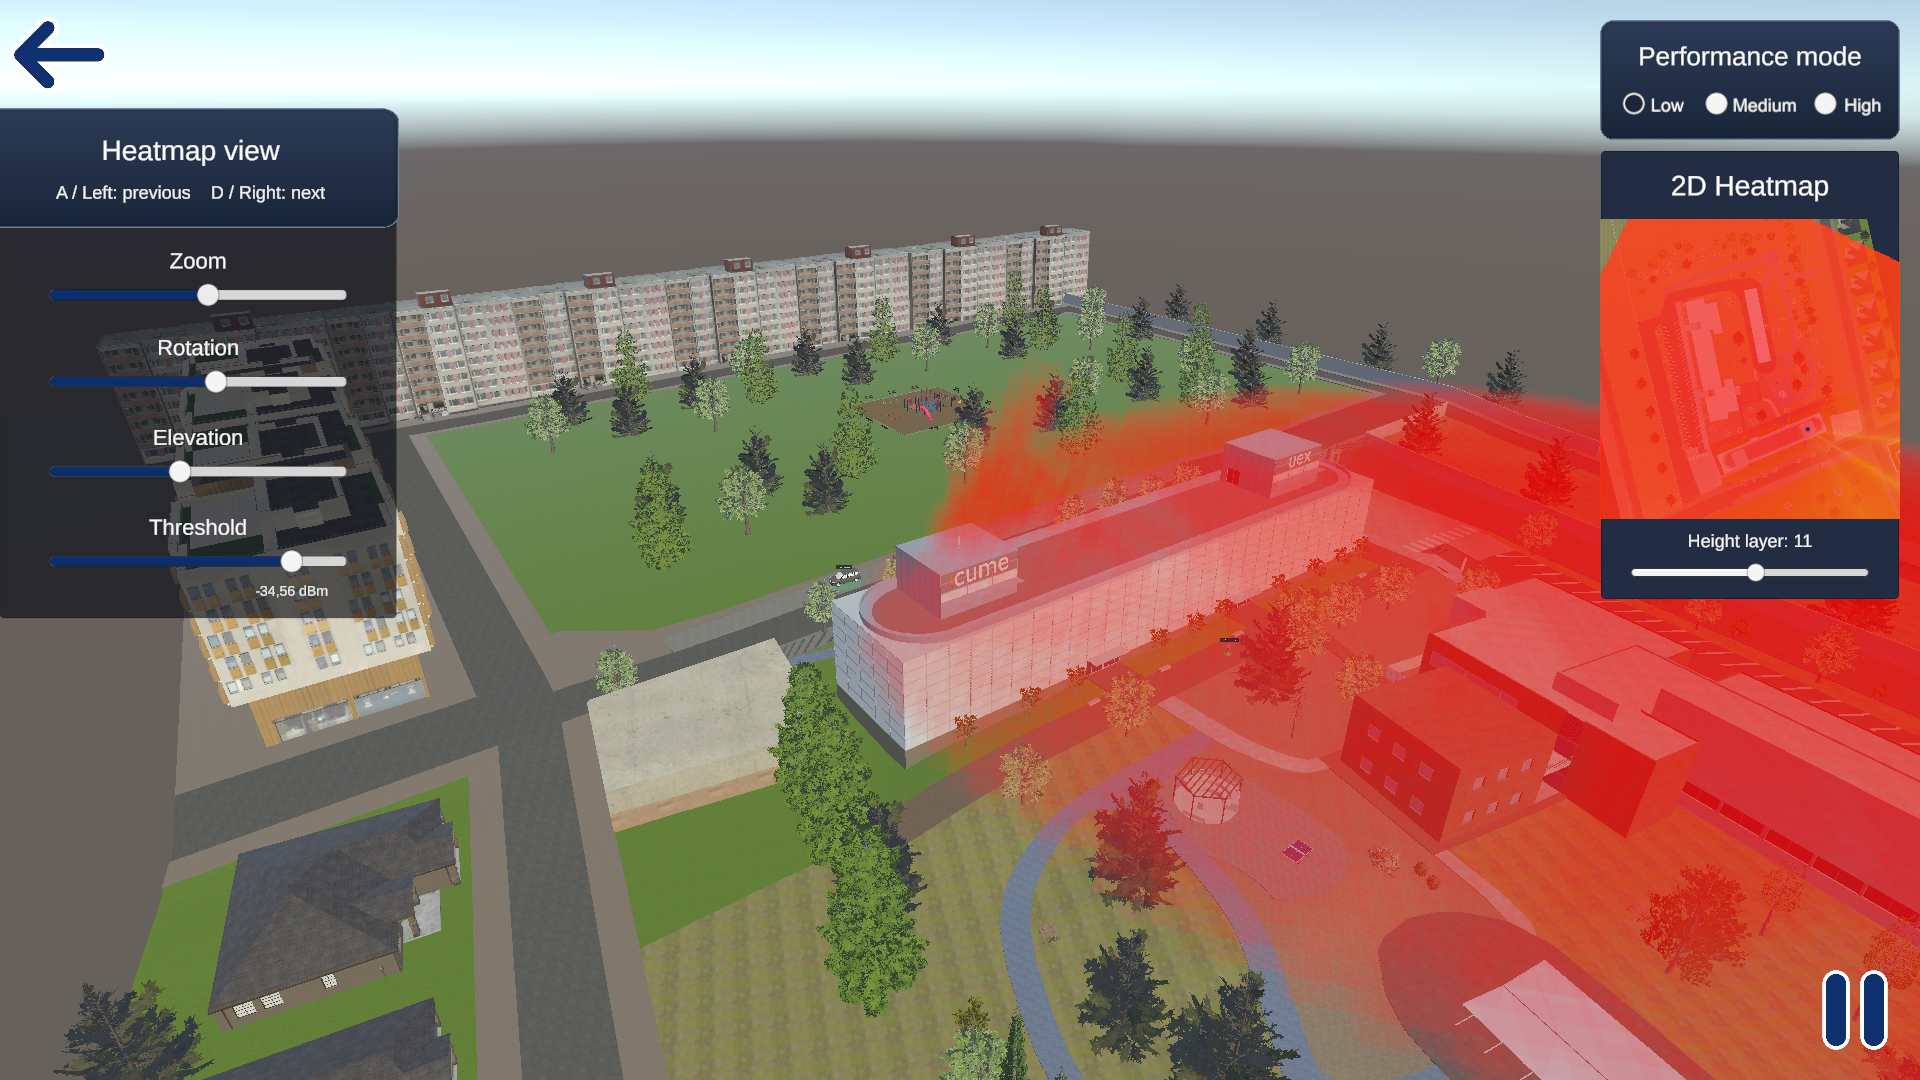
\includegraphics[width=1\textwidth, keepaspectratio]{imagenes/resultados/mapas de calor/Mapa de calor saturado con umbral.PNG}
    \caption{Mapa de calor 3D de la rejilla completa aplicando umbral de visualización}
    \label{fig:heatmap_3d_umbral}
\end{figure}

Además de la representación tridimensional, se utiliza el mapa de calor 2D por capas para estudiar la cobertura en planos horizontales concretos. Esta vista es muy práctica para analizar la rejilla completa, ya que permite estudiar el comportamiento de la señal a una altura determinada evitando el problema de la superposición de vóxeles.

En la Figura \ref{fig:heatmap_2d_campus} se aprecia con mayor detalle la distribución de potencia recibida sobre el campus. Las zonas próximas a la antena y con trayectorias más despejadas presentan valores más altos, mientras que alrededor de algunos edificios se observa una reducción notable de la potencia. Esta disminución se debe a las pérdidas adicionales introducidas cuando la trayectoria entre el transmisor y el punto receptor atraviesa los \textit{colliders} de los edificios.

\begin{figure}[H]
    \centering
    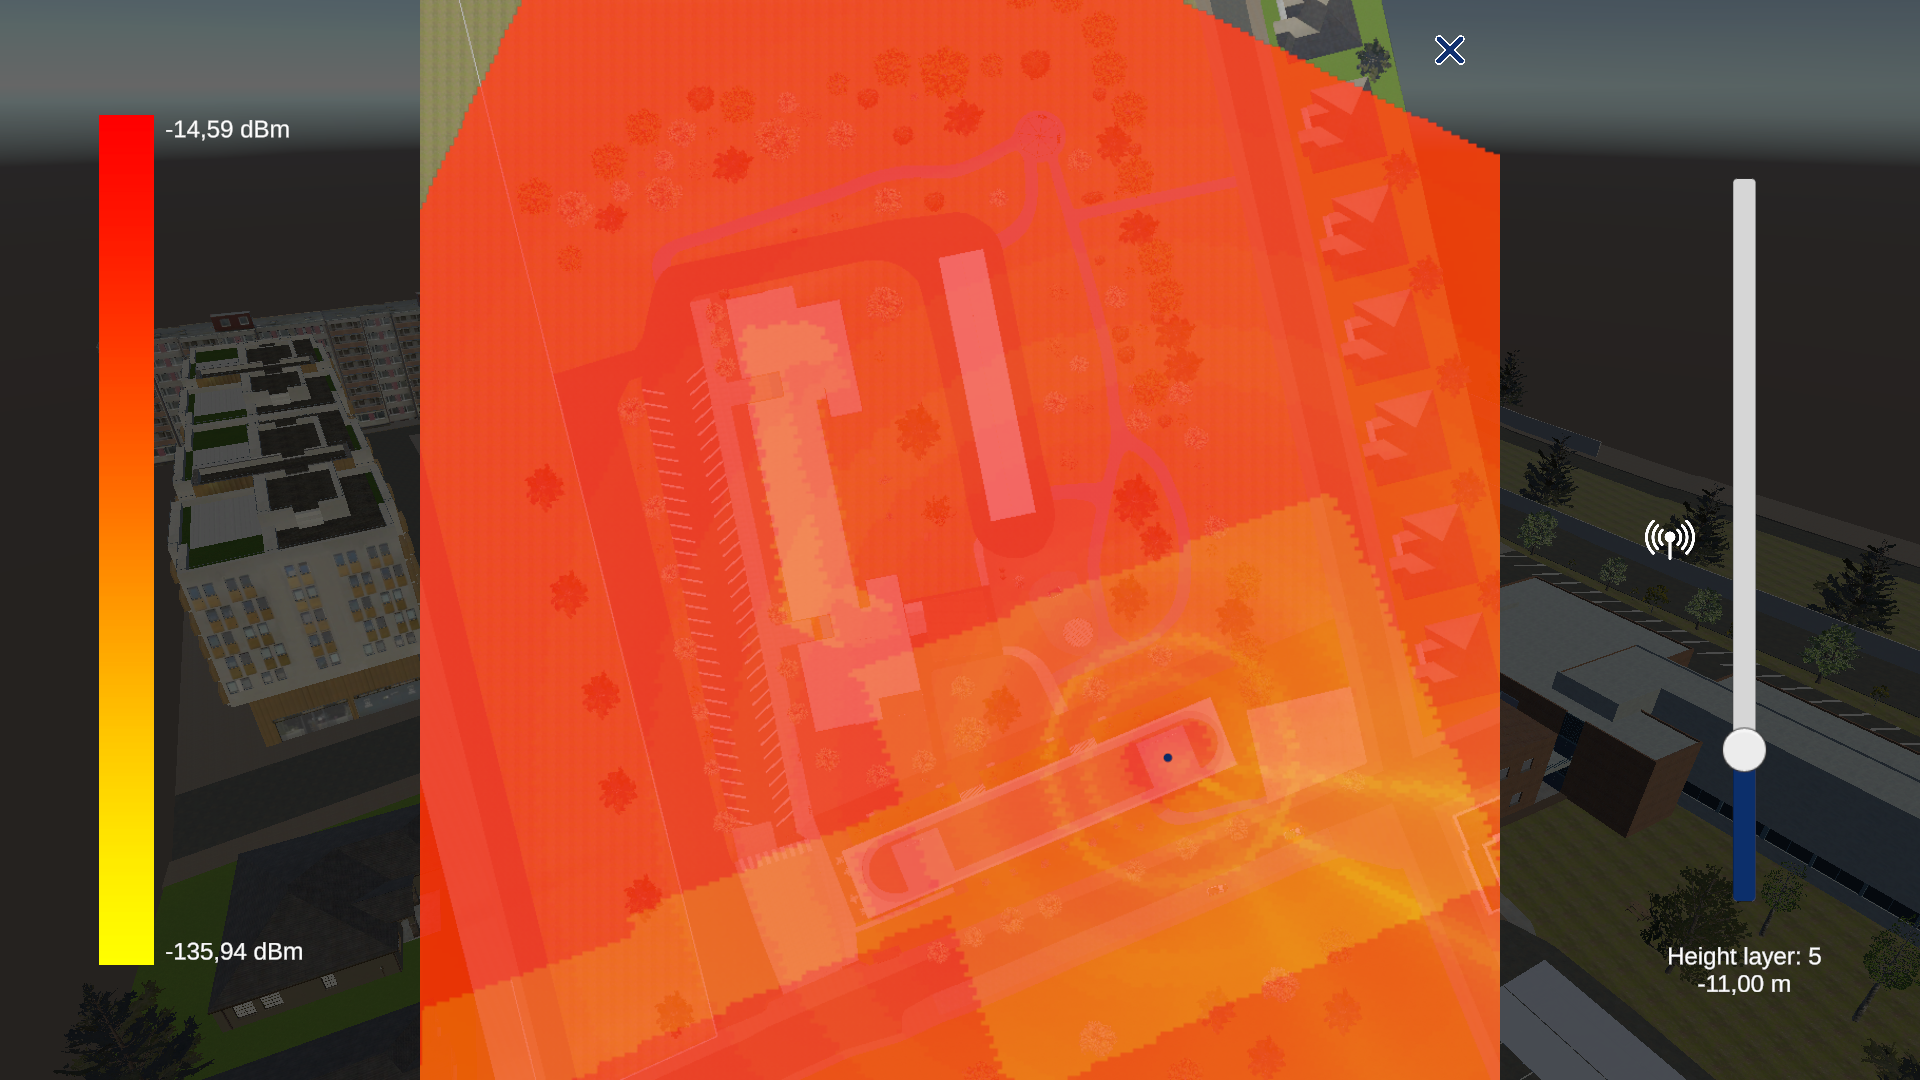
\includegraphics[width=1\textwidth, keepaspectratio]{imagenes/resultados/mapas de calor/Mapa de calor 2D bajo.PNG}
    \caption{Mapa de calor 2D por capas sobre el escenario del campus}
    \label{fig:heatmap_2d_campus}
\end{figure}

Este comportamiento confirma que el mapa de calor no depende únicamente de la distancia a la antena. También influyen la dirección respecto al patrón de radiación y la presencia de obstáculos en el escenario. Por esto, dos puntos situados a la misma distancia del transmisor pueden tener distinta potencia recibida si uno de ellos se encuentra en una zona más alineada con el lóbulo principal o si la señal atraviesa edificios antes de llegar.

En conjunto, estos resultados muestran que la rejilla tridimensional permite obtener una visión general de la cobertura en el campus, mientras que el mapa 2D por capas facilita el análisis detallado de zonas concretas. La combinación de ambas vistas permite interpretar mejor cómo se distribuye la potencia recibida en el escenario y cómo afectan tanto el patrón de radiación como los obstáculos presentes.


\section{Resultados de receptores móviles}

Una vez generada la rejilla de propagación, se activan los receptores móviles y comienzan a actualizarse sus métricas durante el recorrido. En este apartado se muestran los resultados obtenidos con la configuración base, centrándose en la visualización dentro del simulador y en la interpretación de las métricas mostradas en tiempo real.

En las Figuras \ref{fig:metricas_Vehiculo_campus}, \ref{fig:metricas_vehiculo_lineal} y \ref{fig:metricas_peaton} se muestran ejemplos de las vistas asociadas a los tres receptores móviles. Cada vista permite seguir al receptor seleccionado y consultar sus métricas principales, como la distancia al transmisor, la potencia recibida, la SNR, las pérdidas del enlace y el número de colisiones con edificios.

\begin{figure}[H]
    \centering
    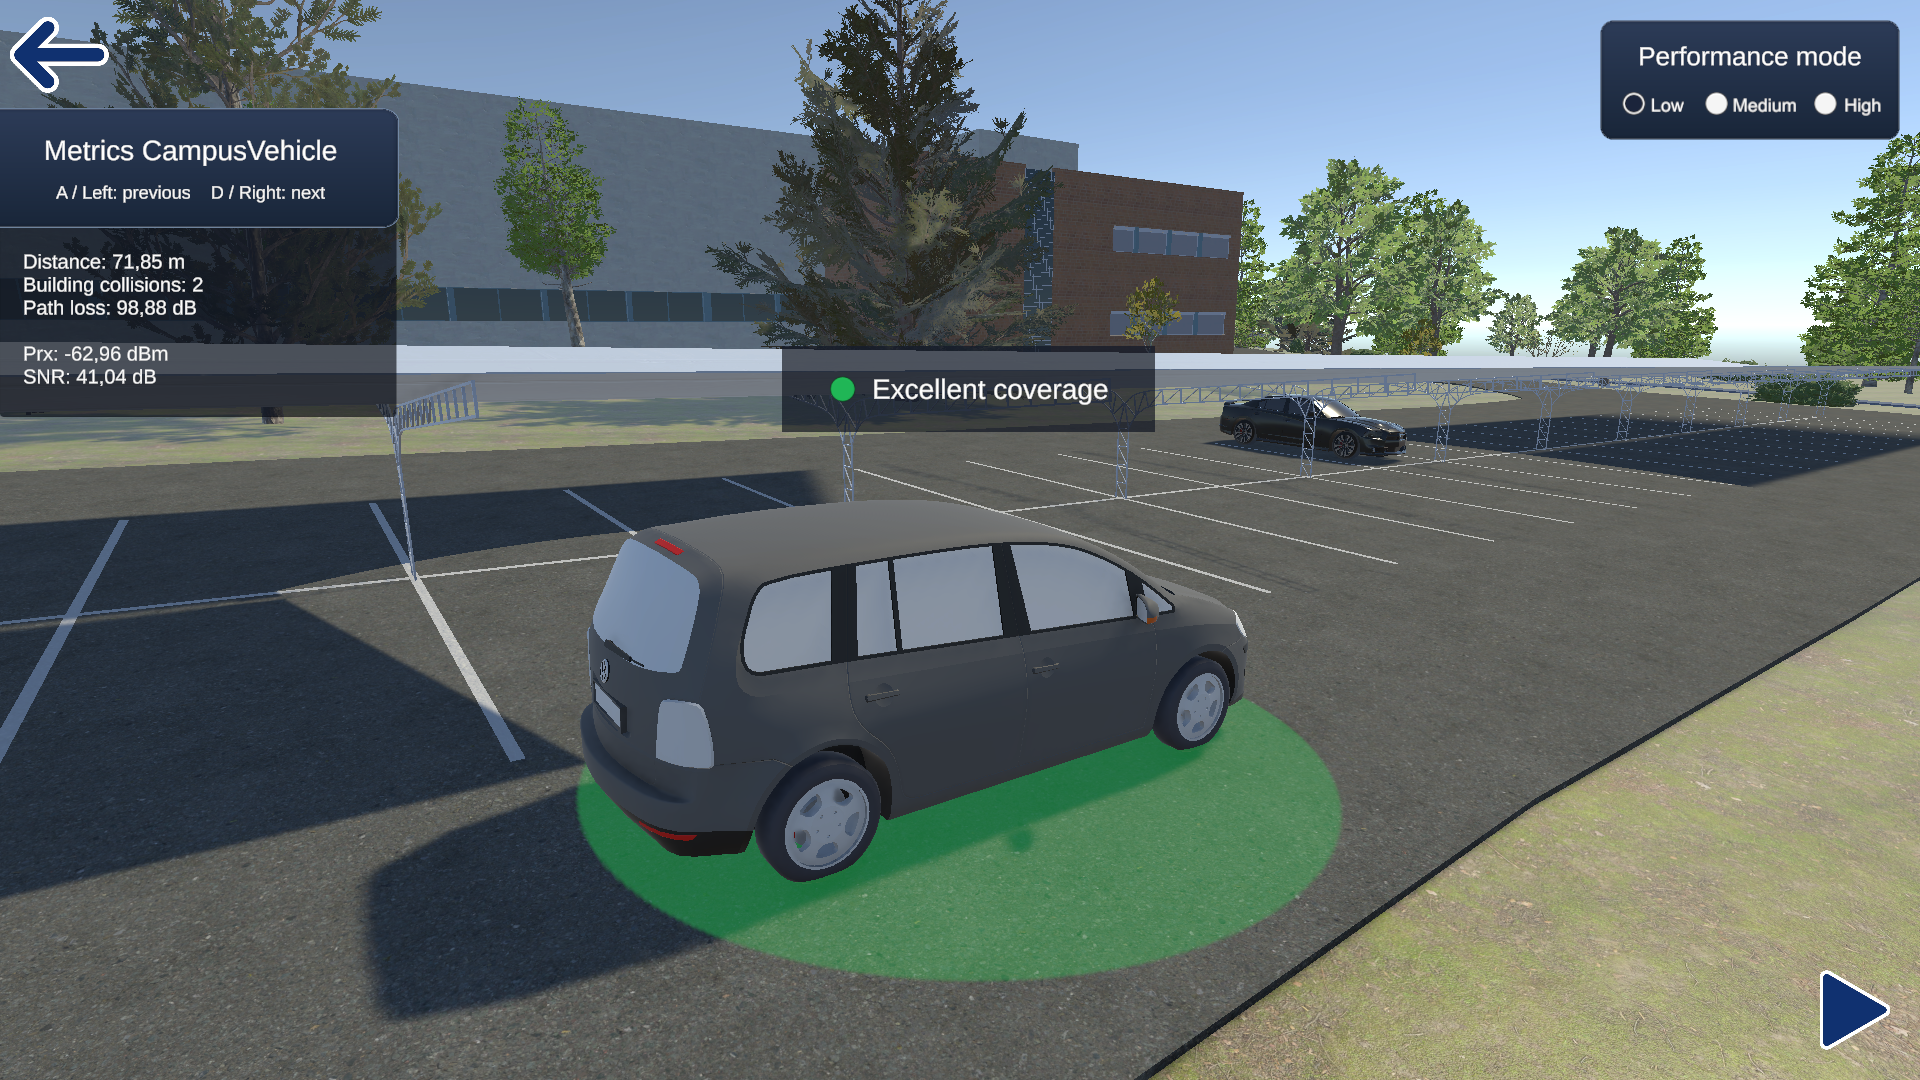
\includegraphics[width=1\textwidth, keepaspectratio]{imagenes/resultados/receptores moviles/vehiculo campus excelente.PNG}
    \caption{Vista del receptor CampusVehicle}
    \label{fig:metricas_Vehiculo_campus}
\end{figure}

\begin{figure}[H]
    \centering
    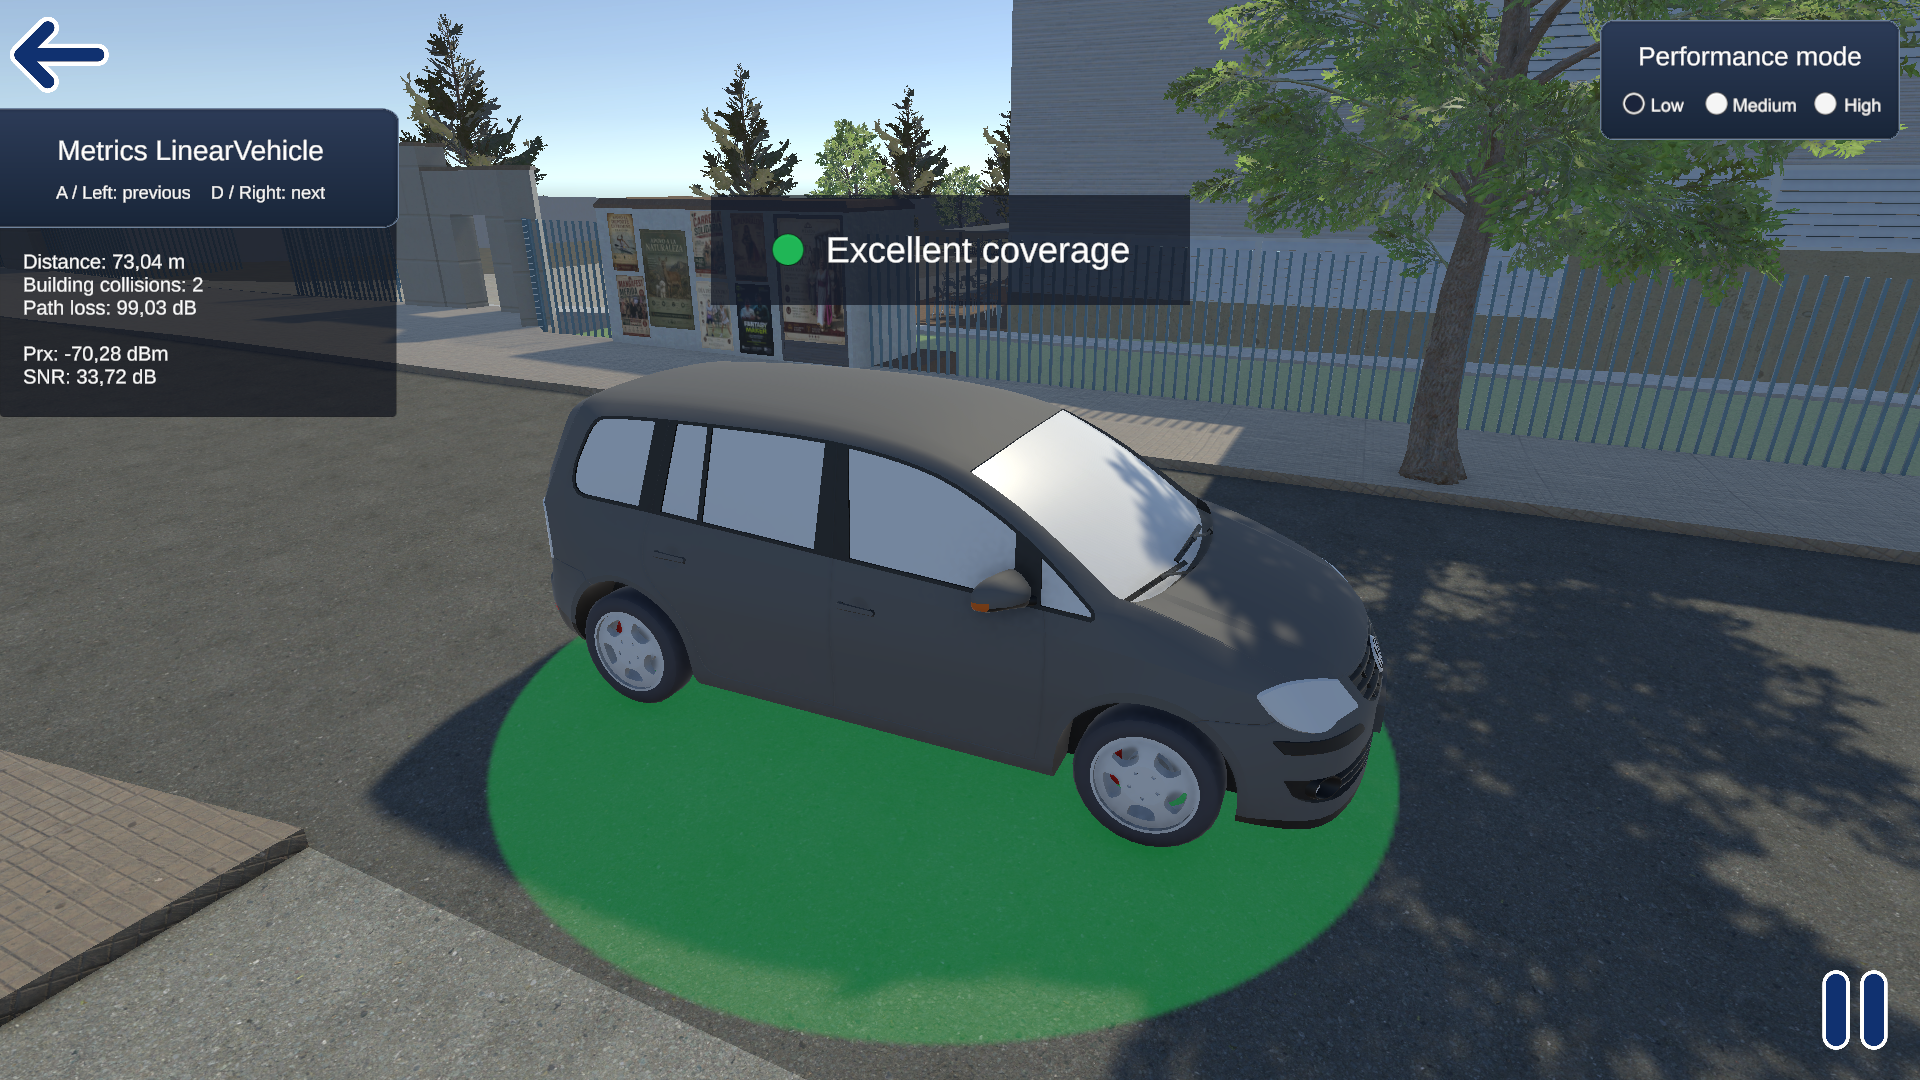
\includegraphics[width=1\textwidth, keepaspectratio]{imagenes/resultados/receptores moviles/vehiculo lineal excelente.PNG}
    \caption{Vista del receptor LinearVehicle}
    \label{fig:metricas_vehiculo_lineal}
\end{figure}

\begin{figure}[H]
    \centering
    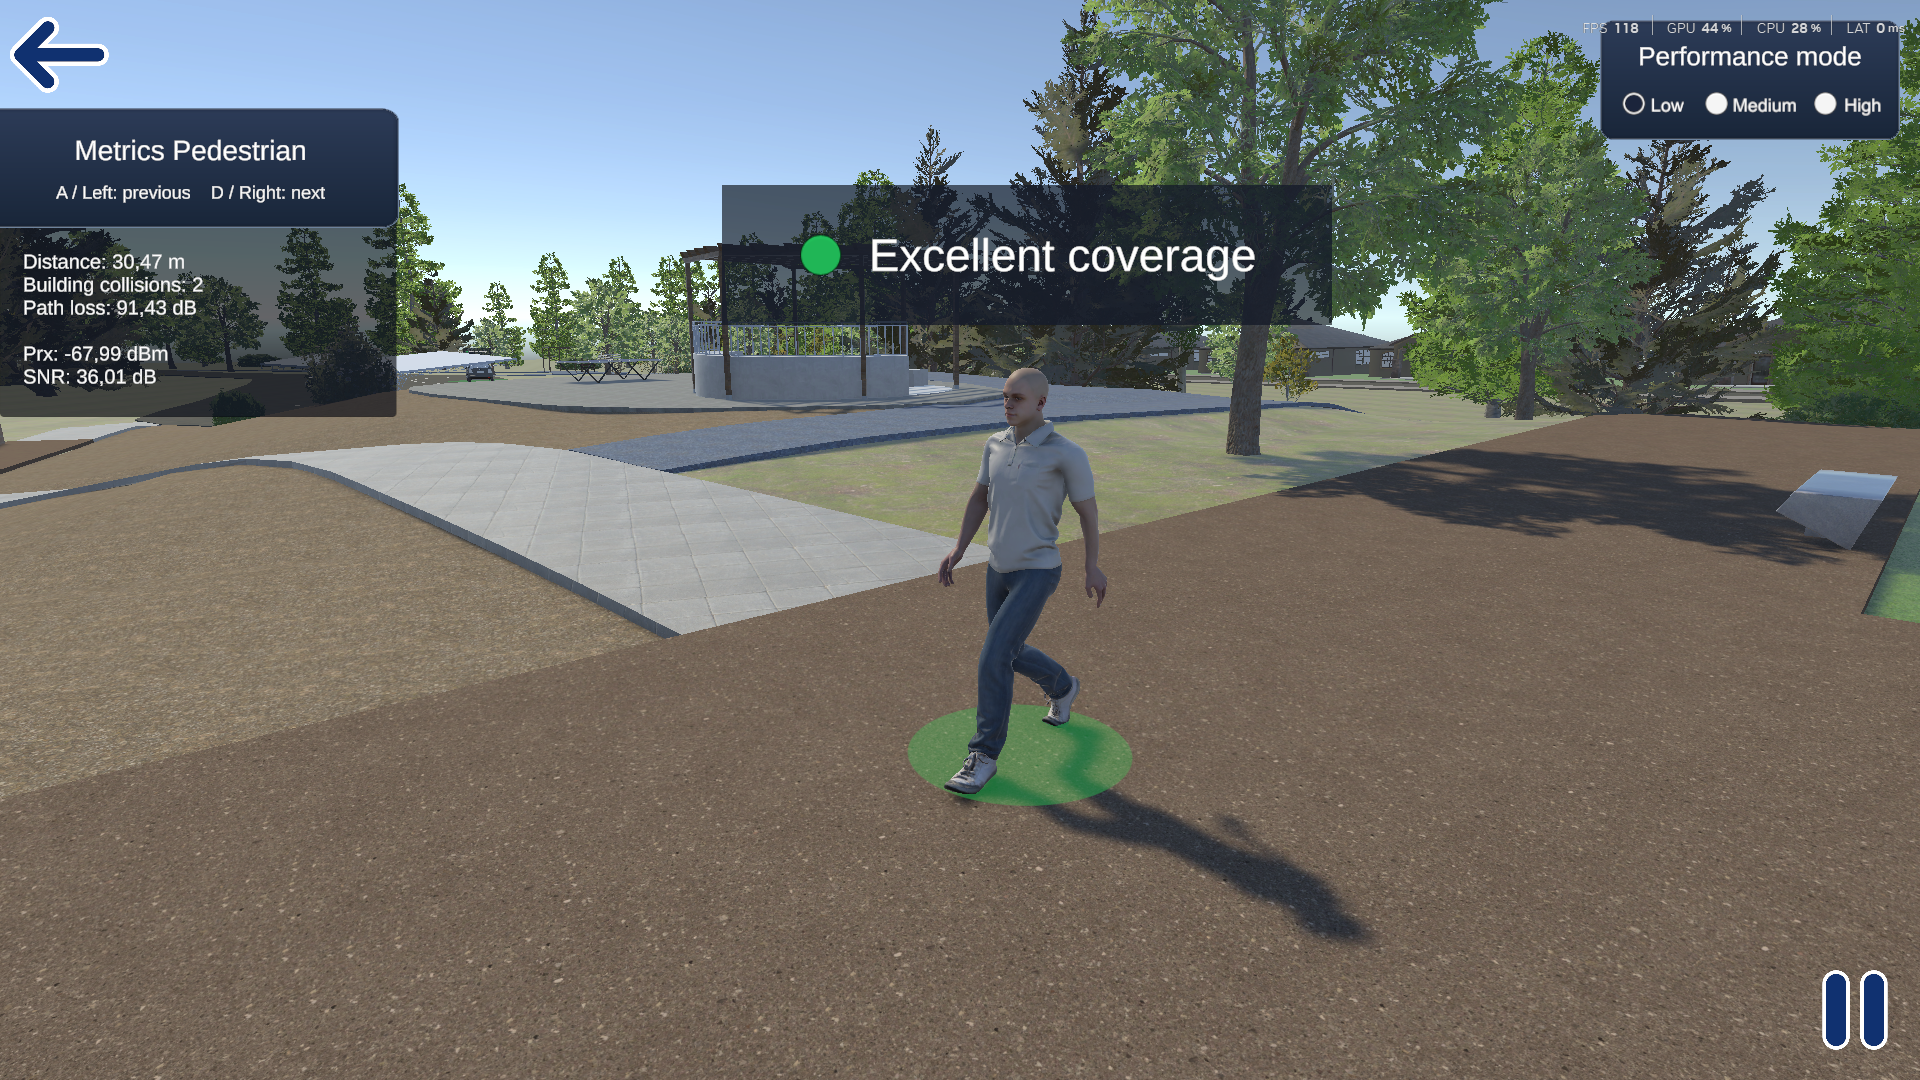
\includegraphics[width=1\textwidth, keepaspectratio]{imagenes/resultados/receptores moviles/peaton excelente.PNG}
    \caption{Vista del receptor Pedestrian}
    \label{fig:metricas_peaton}
\end{figure}

Aunque los tres receptores utilizan la misma configuración de propagación, los valores mostrados no evolucionan de la misma forma. Esto se debe a que cada receptor se desplaza por una zona distinta del escenario y, por tanto, cambia su distancia al transmisor, su orientación respecto al patrón de radiación y el número de obstáculos que la señal atraviesa. Además, los receptores vehiculares utilizan una ganancia de recepción mayor que la del receptor peatonal, lo que también influye en la potencia recibida.

Durante el recorrido, aparece un caso puntual en el que la cobertura cae de forma muy clara. En la Figura \ref{fig:receptor_baja_cobertura} se muestra ese instante. Aunque apenas dura un segundo, resulta interesante porque permite ver cómo el simulador responde cuando se juntan varias condiciones desfavorables en el mismo punto.

En ese momento, la señal atraviesa varios edificios antes de llegar al receptor, por lo que el número de colisiones detectadas es elevado, dando lugar a mayores pérdidas. Además, la dirección entre la antena y el receptor no coincide con una zona de alta ganancia del patrón de radiación. Por eso, la potencia recibida y la SNR bajan de forma considerable, y el indicador visual pasa a mostrar un peor estado de cobertura.

\begin{figure}[H]
    \centering
    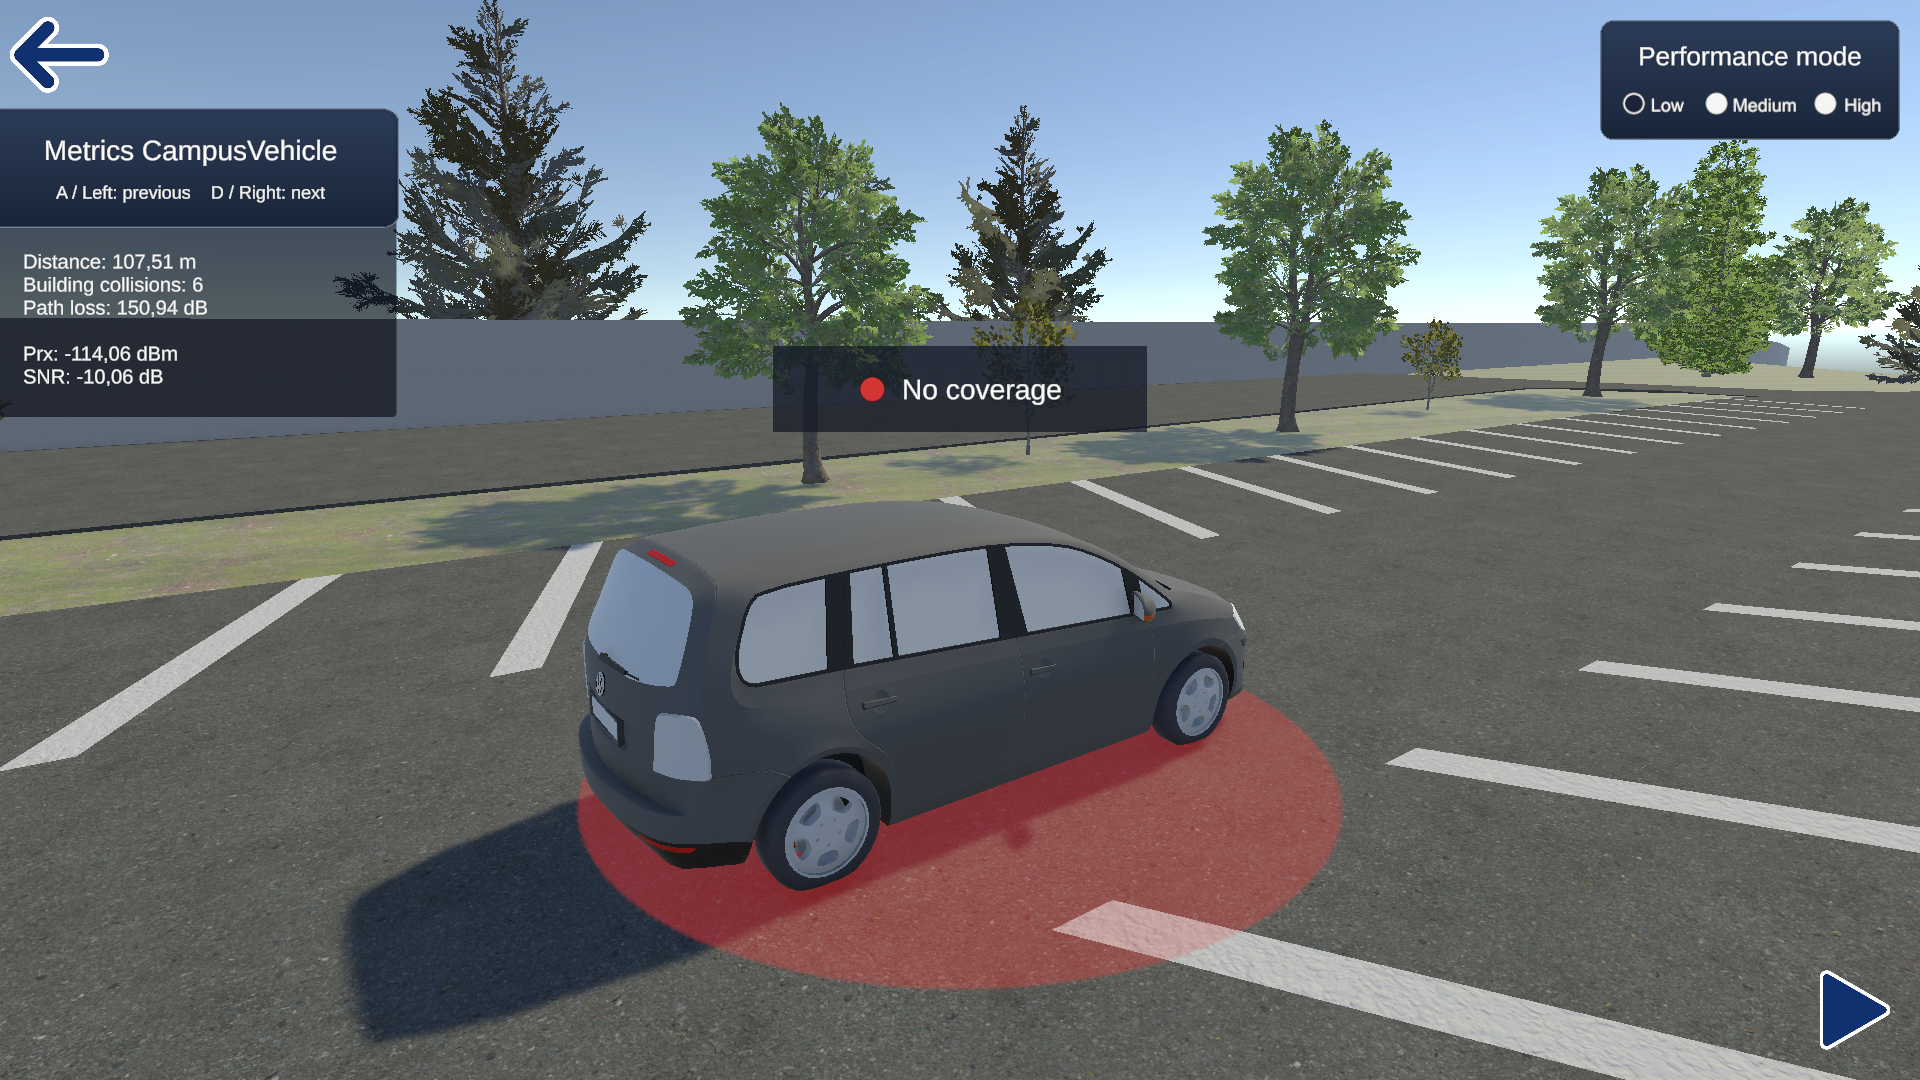
\includegraphics[width=1\textwidth, keepaspectratio]{imagenes/resultados/receptores moviles/vehiculo campus sin cobertura.PNG}
    \caption{Ejemplo de receptor móvil con baja cobertura por obstáculos}
    \label{fig:receptor_baja_cobertura}
\end{figure}

Disponer de un simulador en tres dimensiones permite relacionar los valores numéricos con la posición del receptor dentro del escenario. De esta forma, además de analizar la reducción de potencia en una gráfica, también se puede ver en qué zona del campus se encuentra el receptor y qué elementos del entorno pueden estar afectando al enlace.

Además de mostrar las métricas en tiempo real, el simulador registra los valores calculados durante el recorrido y los exporta posteriormente en archivos CSV. A partir de estos datos se pueden generar gráficas para analizar la evolución de cada receptor. Como ejemplo, en la Figura \ref{fig:linear_vehicle_prx_distance} se muestra la potencia recibida frente a la distancia para el receptor vehicular lineal.

\begin{figure}[H]
    \centering
    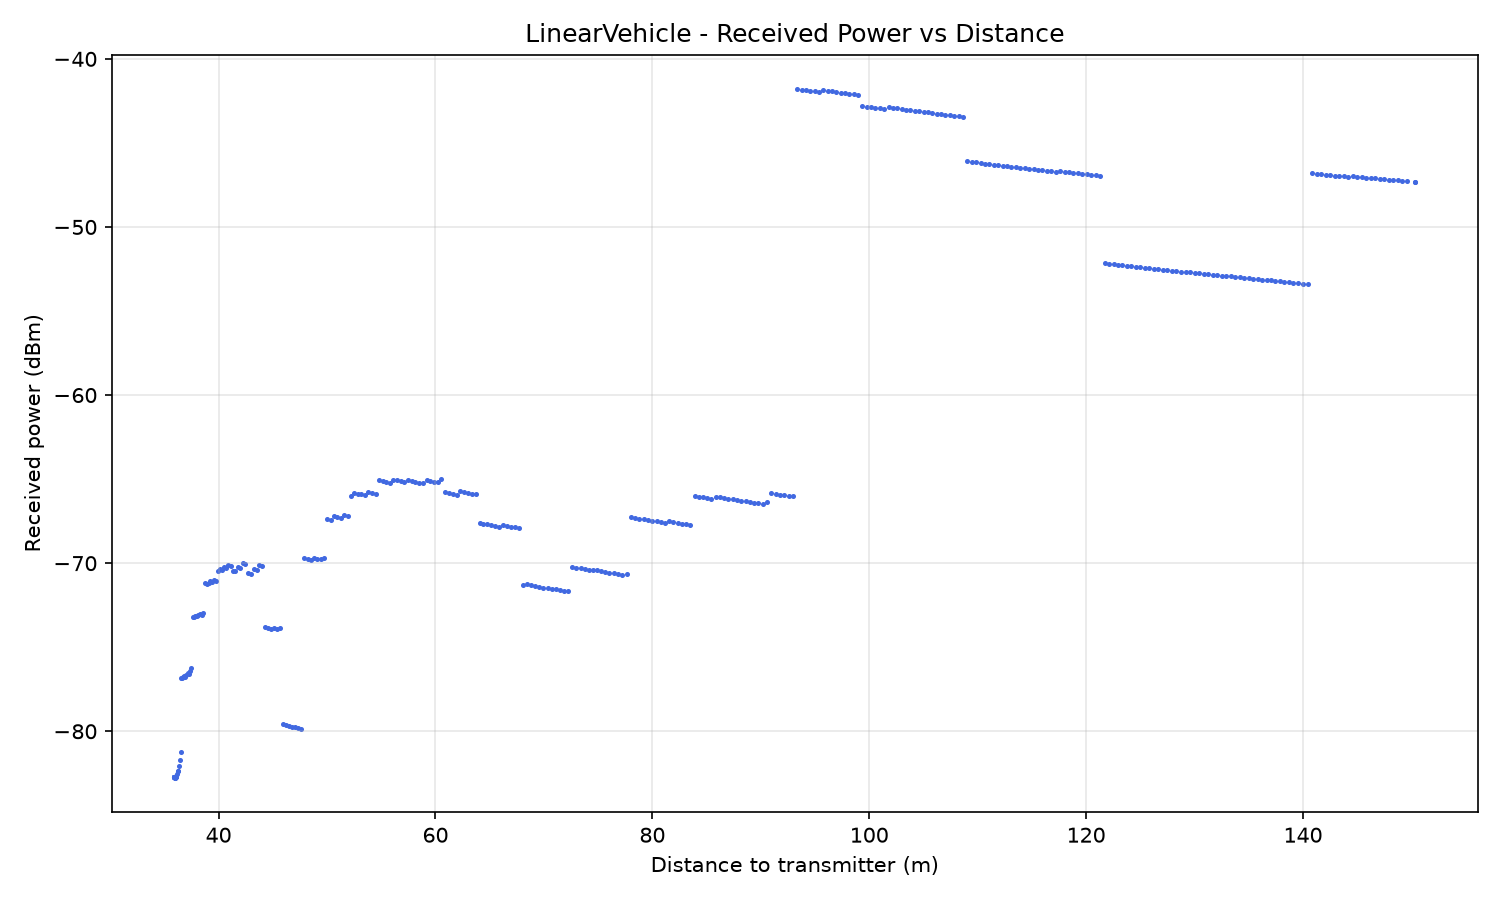
\includegraphics[width=1\textwidth, keepaspectratio]{imagenes/resultados/receptores moviles/30 dbm/LinearVehicle_prx_distance.png}
    \caption{Potencia recibida frente a distancia para el receptor LinearVehicle}
    \label{fig:linear_vehicle_prx_distance}
\end{figure}

En esta gráfica no se observa una disminución uniforme de la potencia recibida con la distancia. Para distancias inferiores a unos 95 m, la señal atraviesa el edificio situado bajo la antena, lo que implica pérdidas adicionales y reduce la potencia recibida. A partir de esa distancia, el receptor deja de estar afectado por esa colisión, y la potencia aumenta de forma brusca. Desde ese punto, la evolución vuelve a ser más progresiva y la potencia tiende a disminuir conforme aumenta la distancia al transmisor. Los saltos menores que aparecen en la gráfica se deben principalmente a los cambios de dirección respecto al patrón de radiación de la antena.

Por tanto, los receptores móviles permiten analizar la cobertura desde dos puntos de vista complementarios. Por un lado, las vistas del simulador muestran en tiempo real la posición del receptor y sus métricas de enlace. Por otro lado, los datos exportados permiten estudiar posteriormente la evolución de esas métricas durante el recorrido. En el siguiente apartado se utiliza esta información para analizar la cobertura según la SNR y los umbrales definidos.

\par\medskip
\textbf{Nota: No sé qué más analizar aquí, tengo varias gráficas aparte de esa pero sería muy repetitivo. Si hay algo más que se os ocurra decídmelo y lo meto.}
\par\medskip


\section{Análisis de cobertura según SNR}

Una vez comprobado el funcionamiento de los receptores móviles, se analiza la cobertura obtenida durante sus recorridos a partir de sus valores de SNR en el tiempo. En este apartado se estudian los resultados de la configuración base y, posteriormente, se aumenta la potencia de transmisión para comparar los cambios en la cobertura resultante.

La comparación se realiza modificando únicamente la potencia de transmisión. Para ello, se utilizan dos valores: 30 dBm, equivalente a 1 W, y 38 dBm, equivalente a 6,31 W. Este último valor corresponde al límite superior definido para una estación base de rango medio según ETSI TS 138 104 \cite{etsi138104}.

Para interpretar los resultados se utilizan los umbrales de SNR configurados en el simulador. En la Figura \ref{fig:snr_time_30dbm} se muestra la evolución temporal de la SNR para el receptor vehicular que recorre el campus utilizando la configuración base de 30 dBm. Se ha elegido este receptor porque su recorrido atraviesa distintas zonas del escenario, dando lugar a más variaciones de cobertura que el resto de receptores móviles.

\begin{figure}[H]
    \centering
    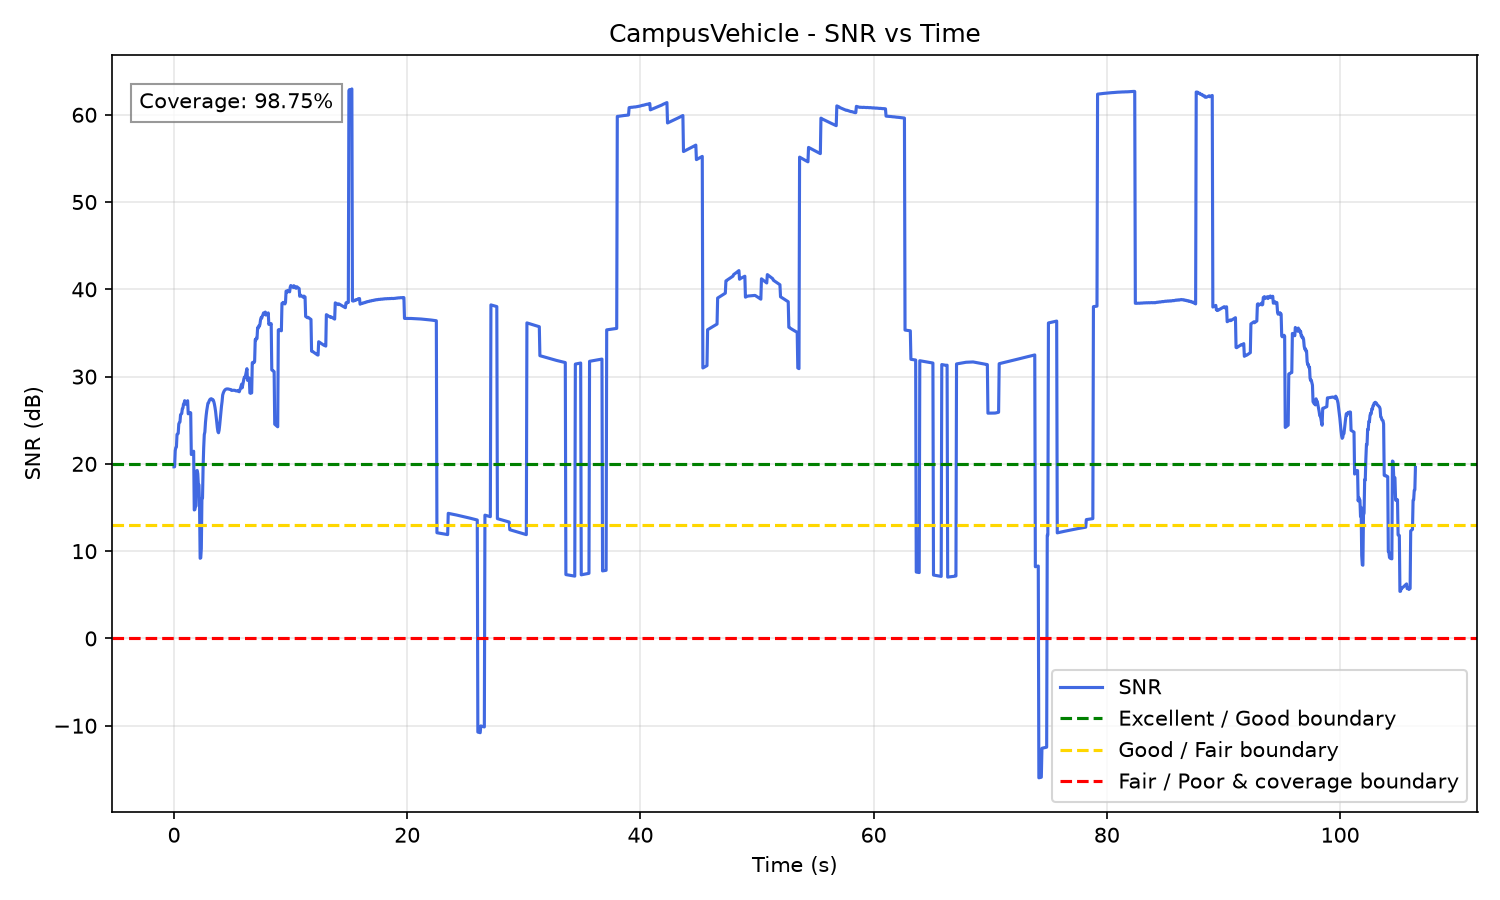
\includegraphics[width=1\textwidth, keepaspectratio]{imagenes/resultados/receptores moviles/30 dbm/CampusVehicle_snr_time.png}
    \caption{Evolución temporal de la SNR con potencia de transmisión de 30 dBm}
    \label{fig:snr_time_30dbm}
\end{figure}

Como se observa, la SNR no se mantiene constante durante el recorrido. Sus variaciones se deben a los cambios de distancia respecto al transmisor, a la orientación respecto al patrón de radiación y a las pérdidas adicionales por las colisiones con edificios.

Al aumentar la potencia de transmisión hasta 38 dBm, la potencia recibida aumenta en todos los puntos del recorrido y, como consecuencia, también mejora la SNR. En la Figura \ref{fig:snr_time_38dbm} se muestra la evolución temporal de la SNR para el mismo receptor utilizando esta potencia superior.

\begin{figure}[H]
    \centering
    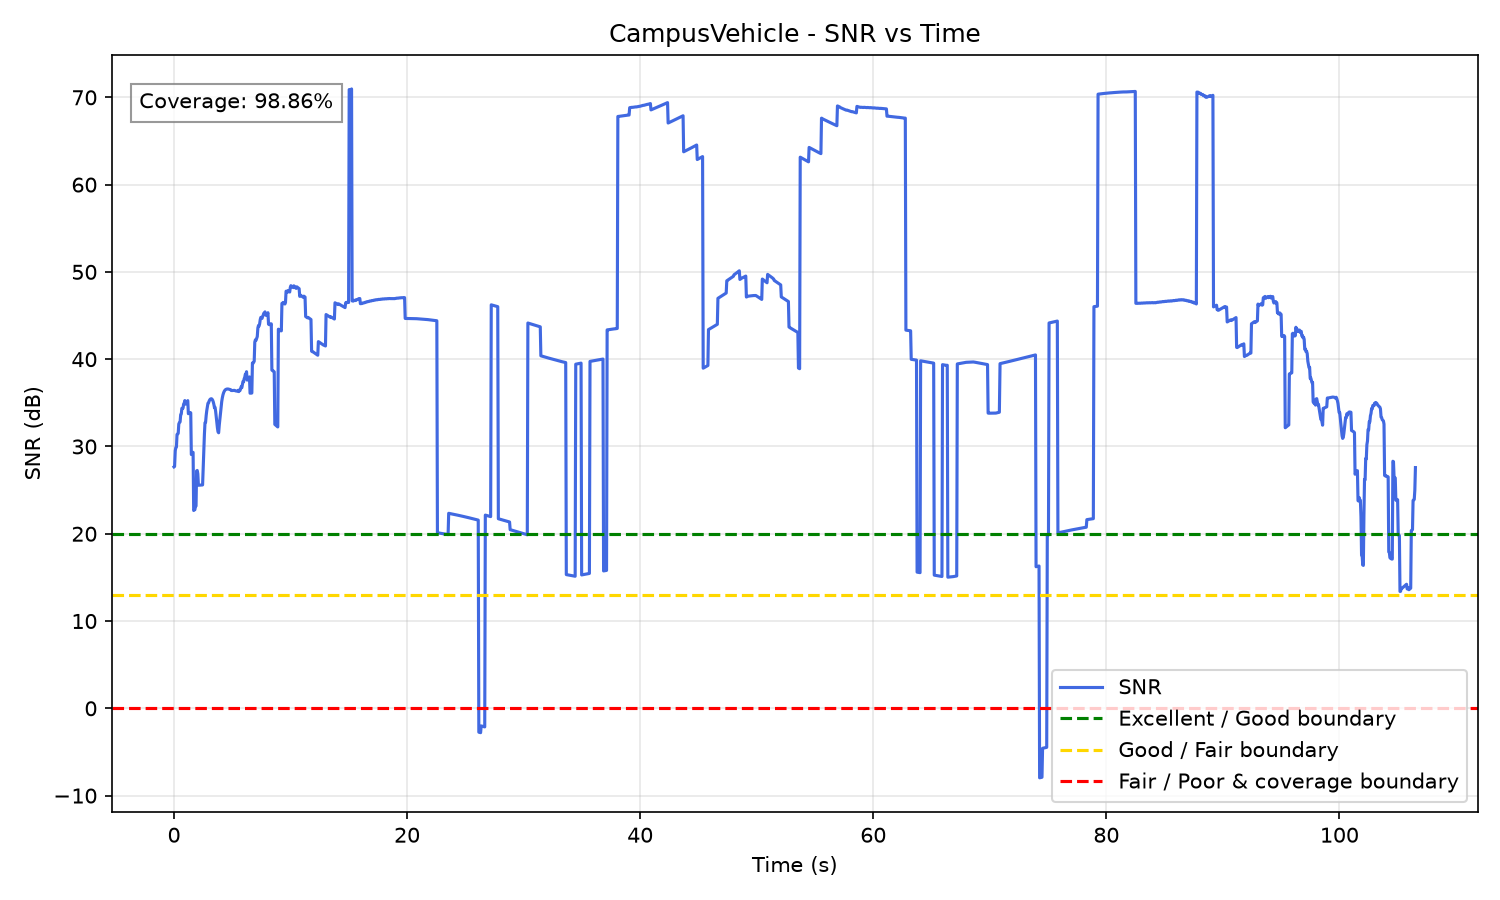
\includegraphics[width=1\textwidth, keepaspectratio]{imagenes/resultados/receptores moviles/38 dbm/CampusVehicle_snr_time.png}
    \caption{Evolución temporal de la SNR con potencia de transmisión de 38 dBm}
    \label{fig:snr_time_38dbm}
\end{figure}

La comparación entre ambas gráficas muestra que el aumento de potencia eleva la SNR durante todo el recorrido. Esto reduce los tramos con cobertura insuficiente y aumenta el porcentaje de tiempo en el que el receptor se mantiene por encima del umbral de cobertura. Sin embargo, las zonas más desfavorables siguen siendo visibles, ya que los obstáculos y las direcciones de menor ganancia del patrón de radiación continúan afectando al enlace.

En la Tabla \ref{tab:cobertura_snr} se muestra el porcentaje de tiempo con cobertura para los tres receptores móviles. Este porcentaje se calcula a partir de las muestras registradas durante el recorrido, considerando como cobertura los instantes en los que la SNR es superior al umbral mínimo establecido anteriormente.

\begin{table}[H]
    \centering
    \begin{tabularx}{\textwidth}{@{}lXX@{}}
        \toprule
        \textbf{Receptor} & \textbf{Cobertura con 30 dBm} & \textbf{Cobertura con 38 dBm}\\
        \midrule
        CampusVehicle & 98,75 \% & 98,86 \% \\
        LinearVehicle & 100 \% & 100 \% \\
        Pedestrian & 100 \% & 100 \% \\
        \bottomrule
    \end{tabularx}
    \caption{Porcentaje de tiempo con cobertura según la SNR}
    \label{tab:cobertura_snr}
\end{table}

Los resultados muestran que, con la configuración base de 30 dBm, la cobertura ya es prácticamente completa en los tres receptores. Tanto el vehículo lineal como el peatón se mantienen por encima del umbral durante todo el recorrido, mientras que el vehículo del campus presenta una pequeña pérdida de cobertura en algunos instantes puntuales. Al aumentar la potencia hasta 38 dBm, esta pérdida se reduce ligeramente, pasando de un 98,75 \% a un 98,86 \%.

La mejora no es muy elevada porque el porcentaje de tiempo con cobertura inicial ya era alto. En este caso, aumentar la potencia no cambia de forma significativa el resultado, pero sí permite comprobar que los puntos más desfavorables del recorrido del vehículo del campus están relacionados con zonas concretas donde coinciden obstáculos y menor ganancia del patrón de radiación. Para eliminar por completo esas caídas, sería necesario seguir aumentando la potencia, aunque esto llevaría a valores menos razonables para el escenario analizado.

Por tanto, este análisis muestra que la configuración base ofrece cobertura suficiente en la mayor parte del campus. La SNR permite detectar los instantes puntuales en los que la cobertura empeora, aunque el porcentaje total siga siendo muy alto. Esto resulta útil porque permite localizar zonas problemáticas que podrían pasar desapercibidas si solo se analizara un valor medio o una visión general del mapa de calor.


\section{Comparación entre configuraciones}

En este apartado se comparan distintas configuraciones del simulador para estudiar cómo afectan algunos parámetros al resultado final. En primer lugar, se analiza el efecto del patrón de radiación utilizado por la antena. Después, se compara el comportamiento obtenido al utilizar dos modelos de pérdidas distintos: FSPL y ABG.

\subsection{Comparación entre patrones de radiación}

Para realizar la comparación, solo se modifica el patrón de radiación utilizado por el simulador. Se utilizan tres patrones diferentes: omnidireccional con ganancia máxima de 16 dBi, reconstrucción mediante el método de Gil y reconstrucción mediante el método de Vasiliadis con $k = 2$.

En la Figura \ref{fig:comparativa_patrones_altura_antena} se muestran los mapas de calor 2D obtenidos para los tres patrones en la capa más cercana a la altura de la antena. Esta comparación permite estudiar cómo varía la distribución de potencia recibida cuando se modifica el patrón de radiación de la antena.

\begin{figure}[H]
    \centering
    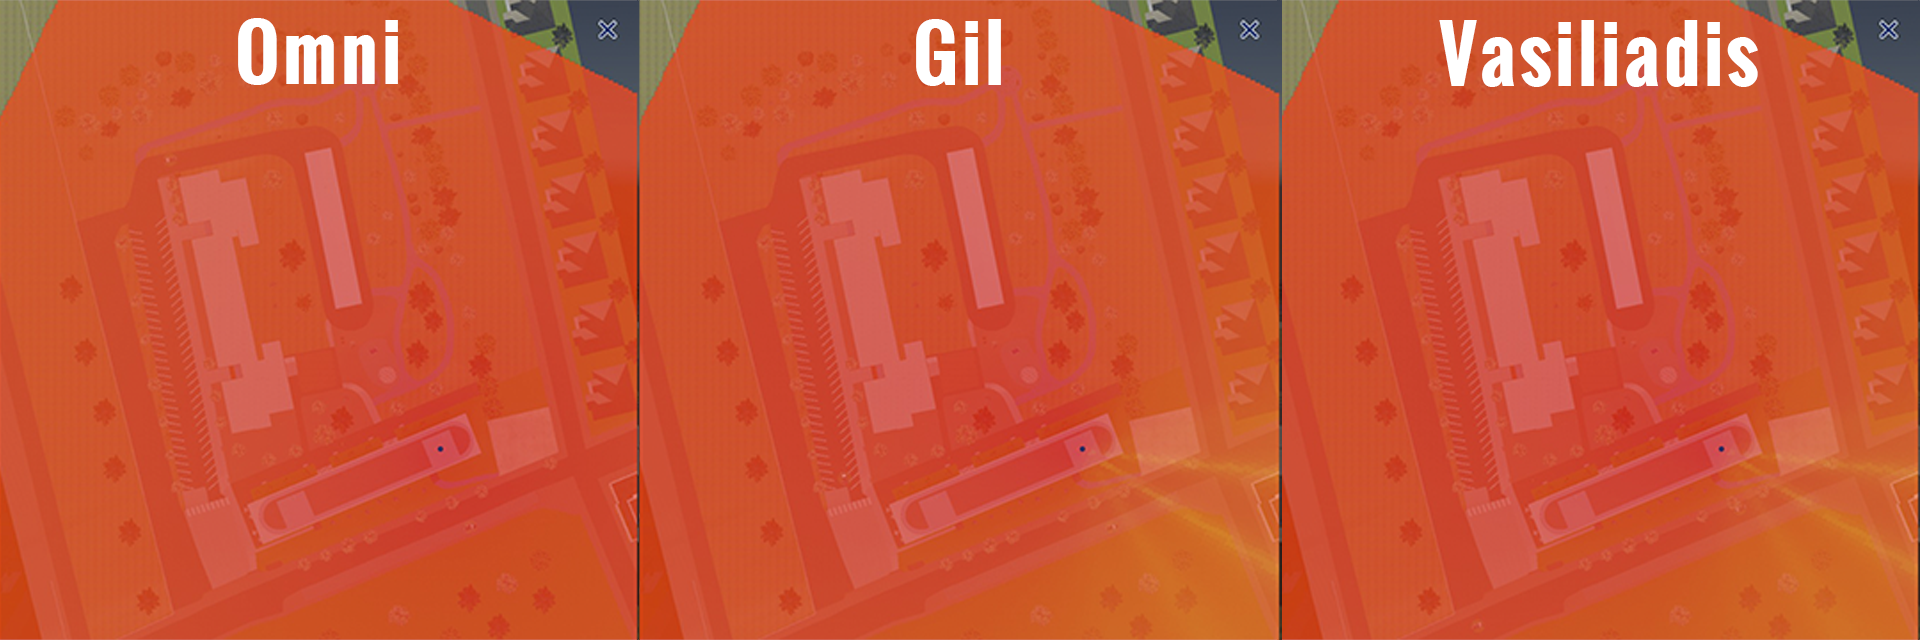
\includegraphics[width=1\textwidth, keepaspectratio]{imagenes/resultados/Comparacion configuraciones/comparacion patrones/comparacion mapas 2d base.png}
    \caption{Comparación de mapas de calor 2D para distintos patrones de radiación a la altura de la antena}
    \label{fig:comparativa_patrones_altura_antena}
\end{figure}

\par\medskip
\textbf{Nota: He puesto dos alturas porque, si no, lo saturaría demasiado de imágenes, aunque lo mejor es verlo en el propio programa y no mediante capturas. Las he recortado para meter tres en una, pero eso hace que no se vea la leyenda, que es un factor importante. La otra opción es poner las tres imágenes completas, una tras otra, pero creo que eso lo saturaría demasiado.}
\par\medskip


En esta capa, las diferencias entre configuraciones son menos evidentes, ya que se trata de una zona cercana a la altura del transmisor y los valores de potencia recibida son elevados en gran parte del mapa. Aun así, se aprecia que el patrón omnidireccional tiene valores altos en todas las direcciones, mientras que los patrones reconstruidos concentran la mayor potencia hacia la parte frontal de la antena. En la zona trasera, tanto Gil como Vasiliadis muestran valores menores, ya que la ganancia del patrón real es menor en dicha dirección.

Para comparar una zona más realista, en la Figura \ref{fig:comparativa_patrones_suelo} se muestra una capa situada cerca del nivel del suelo. Esta altura es más interesante porque se aproxima a la zona donde se encuentran los receptores móviles durante sus recorridos.

\begin{figure}[H]
    \centering
    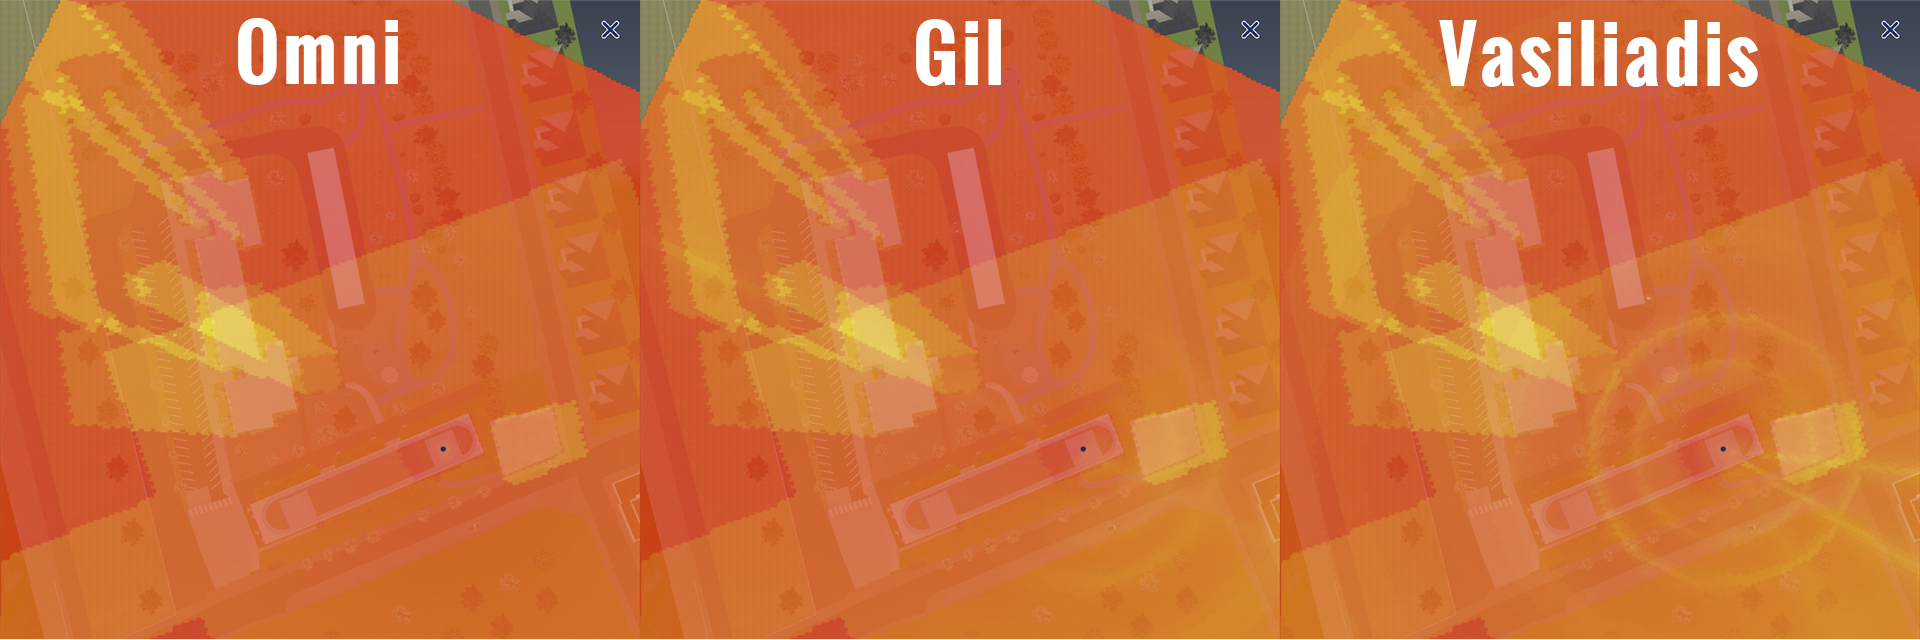
\includegraphics[width=1\textwidth, keepaspectratio]{imagenes/resultados/Comparacion configuraciones/comparacion patrones/comparacion mapas 2d suelo.png}
    \caption{Comparación de mapas de calor 2D para distintos patrones de radiación cerca del nivel del suelo}
    \label{fig:comparativa_patrones_suelo}
\end{figure}

\par\medskip
\textbf{Nota: Realmente no es la altura del suelo, porque al tener un escenario con relieve, el receptor del campus se mueve entre -19 y -25 metros respecto a la antena. Elegí 20 porque es la altura de los otros dos receptores móviles, pero es una aproximación.}
\par\medskip

En la capa cercana al suelo se observan diferencias más claras entre patrones. Con el patrón omnidireccional, la potencia se reparte de forma similar en todas las direcciones, por lo que las zonas de menor potencia se deben a la distancia hasta el transmisor y a las pérdidas introducidas al atravesar edificios.

En cambio, en los patrones reconstruidos aparecen zonas de menor potencia debido a la forma del patrón de radiación. Con Vasiliadis se distinguen varias franjas circulares alrededor de la antena, correspondientes a direcciones con menor ganancia, además de tres haces traseros donde la potencia disminuye de forma notable. En Gil también aparecen variaciones similares, aunque se observan principalmente franjas semicirculares en la parte trasera y con un haz de menor potencia menos marcado.

Además del mapa de calor, se analiza el efecto de cada patrón sobre los receptores móviles. Para ello, se calcula la potencia recibida media durante el recorrido de cada receptor, utilizando los datos exportados en los archivos CSV. Como los valores de potencia están expresados en dBm, primero se convierten a escala lineal en mW, después se calcula la media y finalmente se vuelve a convertir el resultado a dBm. En la Tabla \ref{tab:comparativa_patrones_prx} se muestran los resultados obtenidos para los tres patrones de radiación analizados.

\begin{table}[H]
    \centering
    \begin{tabularx}{\textwidth}{@{}lXXX@{}}
        \toprule
        \textbf{Receptor} & \textbf{Omni} & \textbf{Gil} & \textbf{Vasiliadis} \\
        \midrule
        CampusVehicle & -36,44 dBm & -43,43 dBm & -50,42 dBm \\
        LinearVehicle & -33,94 dBm & -42,91 dBm & -49,87 dBm \\
        Pedestrian & -49,61 dBm & -58,14 dBm & -67,37 dBm \\
        \bottomrule
    \end{tabularx}
    \caption{Potencia recibida media para distintos patrones de radiación}
    \label{tab:comparativa_patrones_prx}
\end{table}

Los resultados permiten comprobar que el patrón de radiación influye fuertemente en la potencia recibida por los receptores móviles. En todos los recorridos, el patrón omnidireccional da lugar a los valores medios más altos. Esto se debe a que, aunque también presenta variación con la elevación, no introduce una diferencia tan marcada entre la parte frontal y trasera de la antena como ocurre con los patrones reconstruidos.

Sin embargo, este resultado no significa que el patrón omnidireccional sea la configuración más realista. Los patrones reconstruidos representan mejor el comportamiento direccional de la antena utilizada, ya que parten de los cortes reales del patrón de radiación. Aunque sus valores medios sean menores, especialmente en el caso de Vasiliadis, estos resultados son más coherentes con una antena real, donde la potencia recibida depende de la dirección concreta en la que se encuentra cada receptor respecto al transmisor.

Por tanto, la comparación muestra que no basta con analizar si existe cobertura o no. Dos configuraciones pueden ofrecer cobertura suficiente en gran parte del recorrido, pero presentar niveles de potencia recibida muy distintos. Por este motivo, la potencia media y los mapas de calor ayudan a interpretar mejor el efecto del patrón de radiación utilizado.

\subsection{Comparación entre modelos de pérdidas}

Además del patrón de radiación, el modelo de pérdidas utilizado también afecta a los resultados obtenidos. Para comprobarlo, se comparan dos configuraciones modificando únicamente el modelo de pérdidas: una utilizando el modelo FSPL y otra utilizando el modelo ABG.

El modelo FSPL representa la propagación en espacio libre, por lo que depende principalmente de la distancia y de la frecuencia. En cambio, el modelo ABG incorpora parámetros dependientes del tipo de escenario y permite representar un comportamiento más específico para entornos urbanos. Por este motivo, se espera que los resultados obtenidos con ABG no coincidan con los obtenidos mediante FSPL.

En la Figura \ref{fig:comparativa_fspl_abg} se muestra la comparación entre ambos modelos de pérdidas para la misma configuración de antena y potencia de transmisión. Para facilitar la interpretación, se utiliza nuevamente la capa más cercana al nivel del suelo.

\begin{figure}[H]
    \centering
    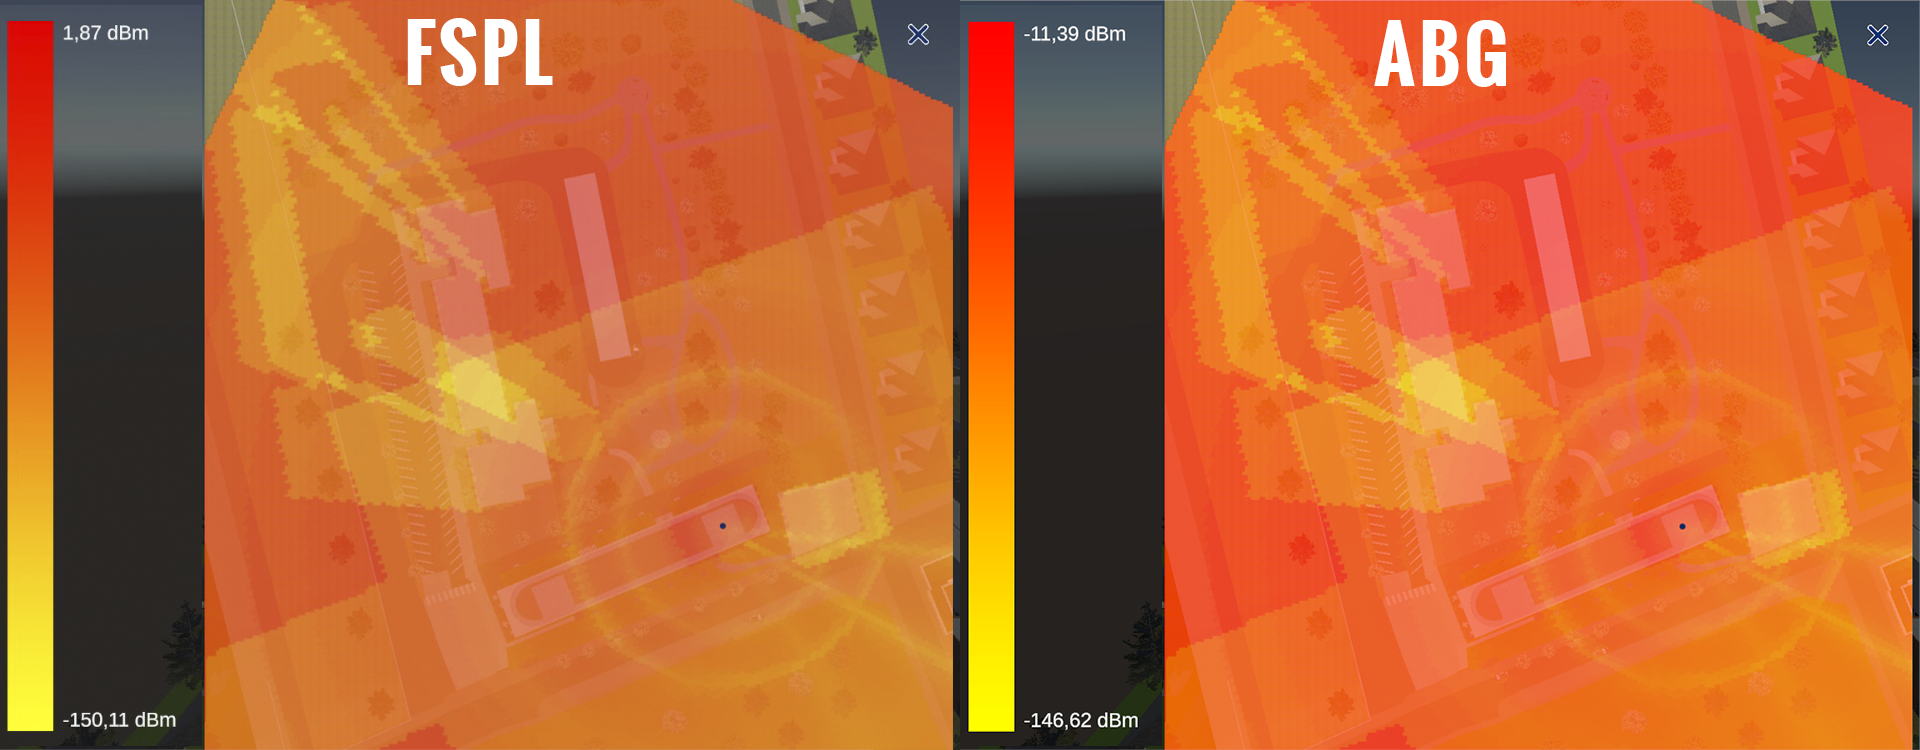
\includegraphics[width=1\textwidth, keepaspectratio]{imagenes/resultados/Comparacion configuraciones/comparacion modelos/Comparacion modelos.png}
    \caption{Comparación de mapas de calor 2D utilizando los modelos FSPL y ABG}
    \label{fig:comparativa_fspl_abg}
\end{figure}

En la comparación visual se observa que la distribución de potencia es similar en ambos modelos. Las zonas de mayor y menor potencia aparecen aproximadamente en las mismas regiones del campus, ya que se mantiene el mismo patrón de radiación, la misma posición de la antena y los mismos obstáculos en el escenario. Sin embargo, los valores límite sí cambian: en FSPL el valor máximo mostrado es de 1,87 dBm, mientras que en ABG es de -11,39 dBm. Los valores mínimos, al contrario, son más cercanos, con -150,11 dBm en FSPL y -146,62 dBm en ABG.

Por tanto, aunque el mapa de calor permite ver que la distribución general es muy similar, no es suficiente para valorar por sí solo cómo afecta el cambio de modelo a los receptores. Para completar la comparación, se calcula la potencia recibida media de cada receptor a partir de los datos exportados en los CSV. Al igual que en el apartado anterior, los valores en dBm se convierten primero a mW, se calcula la media en escala lineal y, finalmente, se vuelve a convertir el resultado a dBm.

\begin{table}[H]
    \centering
    \begin{tabularx}{\textwidth}{@{}lXX@{}}
        \toprule
        \textbf{Receptor} & \textbf{FSPL} & \textbf{ABG} \\
        \midrule
        CampusVehicle & -50,42 dBm & -46,47 dBm \\
        LinearVehicle & -49,87 dBm & -46,10 dBm \\
        Pedestrian & -67,37 dBm & -66,93 dBm \\
        \bottomrule
    \end{tabularx}
    \caption{Potencia recibida media para distintos modelos de pérdidas}
    \label{tab:comparativa_modelos_perdidas}
\end{table}

Los valores de la tabla permiten comparar el efecto de cada modelo sobre los recorridos de los receptores móviles. Aunque en el mapa de calor el valor máximo de ABG es menor que el de FSPL, las potencias medias obtenidas para los receptores vehiculares son superiores con ABG. Esto indica que, aunque el valor máximo del mapa de calor sea mayor, no significa que todas las potencias recibidas lo sean.

En el caso del receptor peatonal, la diferencia entre ambos modelos es mucho menor. Esto se debe a que cada receptor recorre zonas distintas del escenario, con diferentes distancias al transmisor, direcciones respecto al patrón de radiación y colisiones con edificios. Por tanto, el cambio de modelo de pérdidas no afecta por igual a todos los receptores.

Esta comparación muestra que es importante analizar los resultados desde varios puntos de vista. El mapa de calor permite observar la distribución espacial de la potencia, mientras que los datos exportados de los receptores móviles permiten estudiar qué ocurre durante recorridos concretos. Por ello, no es suficiente quedarse solo con la representación visual o con un valor máximo, sino que es necesario combinar ambas fuentes de información.

\par\medskip
\textbf{Nota: He hecho todas las pruebas que hemos ido hablando en las reuniones y que me habéis dicho. Es un poco raro por el tema de que el punto fuerte de este trabajo es la visualización en tiempo real y aquí solo se pueden poner capturas. No obstante, si se os ocurre algo más decídmelo y meto la prueba/datos que me digáis.}
\par\medskip


\section{Limitaciones detectadas}

Aunque el simulador desarrollado permite analizar la cobertura de forma visual y comparar distintas configuraciones, durante las pruebas se han detectado algunas limitaciones que deben tenerse en cuenta al interpretar los resultados:

\begin{itemize}
   \item \textbf{Pérdida asociada a edificios:} las pérdidas por edificios se calculan correctamente a partir de las colisiones detectadas, pero todos los edificios se interpretan como si estuvieran formados únicamente por hormigón. Por tanto, no se diferencian materiales como cristal, metal o ladrillo, ni se tienen en cuenta ventanas, ventanales, puertas o muros interiores. Además, los edificios se consideran huecos, por lo que no se modelan las pérdidas que podrían aparecer al atravesar su interior.
    
    \item \textbf{Resolución de la rejilla de propagación:} para cubrir todo el campus es necesario generar una cantidad de vóxeles muy elevada. Lo ideal sería utilizar un tamaño de vóxel menor para obtener mejores resultados, pero al reducirlo aumentan enormemente los recursos necesarios para llevar a cabo la simulación, pudiendo hacer que deje de ejecutarse correctamente en equipos convencionales. Por este motivo, en las pruebas que cubren todo el campus se utiliza un tamaño de vóxel de 2 m. Este valor permite mantener un coste computacional asumible, pero reduce la resolución de los mapas de calor.

    \item \textbf{Rutas de los receptores móviles:} las métricas de los receptores móviles solo se obtienen en los puntos por los que pasan sus rutas. Esto permite estudiar la evolución de la señal durante recorridos concretos, pero no conocer directamente la potencia recibida en cualquier punto deseado del campus.

    \item \textbf{Reconstrucción aproximada del patrón de radiación:} el patrón tridimensional se obtiene a partir de los dos cortes bidimensionales de la antena. Esto genera una aproximación, pero no equivale a una medida real completa en tres dimensiones. Además, algunos métodos de reconstrucción simplifican la información. Por ejemplo, el método de Vasiliadis trabaja únicamente con 180 grados del patrón, por lo que parte de la información original se pierde durante la reconstrucción.

    \item \textbf{Visualización del mapa de calor:} al representar muchos vóxeles semitransparentes al mismo tiempo, algunas zonas pueden saturarse visualmente y ser difíciles de interpretar. Para reducir este problema, se añadieron controles de transparencia, umbral y mapa 2D por capas, pero la interpretación del mapa sigue dependiendo de la configuración visual elegida por el usuario.
\end{itemize}
